\documentclass[times, utf8, diplomski, numeric]{fer}

\usepackage{booktabs}
\usepackage{listings}

\usepackage{xcolor}
\usepackage{color, colortbl}
\usepackage{pgfplotstable}
\usepackage{pgfplots}

\usepackage{url}
\def\UrlBreaks{\do/\do-}
\usepackage{breakurl}
\usepackage[breaklinks]{hyperref}

\hypersetup{
	colorlinks,
	linkcolor={black},
	citecolor={black},
	urlcolor={black}
}

\definecolor{codegray}{rgb}{0.5,0.5,0.5}
\definecolor{codegreen}{rgb}{0,0.6,0}
\definecolor{codepurple}{rgb}{0.58,0,0.82}
\definecolor{lightblue}{rgb}{0.7,0.99,0.99}
\definecolor{darkblue}{rgb}{0.08,0.41,0.69}

\lstdefinestyle{mystyle}{
	frame=single,   
	commentstyle=\color{codegreen},
	keywordstyle=\color{magenta},
	stringstyle=\color{codepurple},
	basicstyle=\ttfamily,
	breakatwhitespace=false,         
	breaklines=true,                 
	captionpos=b,                    
	keepspaces=true,                 
	showspaces=false,                
	showstringspaces=false,
	showtabs=false,                  
	tabsize=2
}

\lstset{style=mystyle}

\lstdefinelanguage{json}{
	breaklines=true,
	frame=single,
	literate=
	*{:}{{{\color{magenta}{:}}}}{1}
	{,}{{{\color{magenta}{,}}}}{1}
	{\{}{{{\color{darkblue}{\{}}}}{1}
	{\}}{{{\color{darkblue}{\}}}}}{1}
	{[}{{{\color{darkblue}{[}}}}{1}
	{]}{{{\color{darkblue}{]}}}}{1},
}

\lstdefinelanguage{flux}{
	breaklines=true,
	frame=single,
	morekeywords=[1]{from},
	morekeywords=[2]{range, filter, last},
	morekeywords=[3]{group, pivot, keep, drop},
	morekeywords=[4]{count, map, yield},
	keywordstyle=[1]\color{darkblue},
	keywordstyle=[2]\color{blue},
	keywordstyle=[3]\color{magenta},
	keywordstyle=[4]\color{codegreen},
	morestring=[b]",
	stringstyle=\color{codepurple},
	sensitive=true,
	commentstyle=\color{codegray}\ttfamily,
	morecomment=[l]{//},
	morecomment=[s]{/*}{*/}
}


\renewcommand*{\lstlistingname}{Isječak koda}
\renewcommand*\lstlistlistingname{Popis isječaka koda}

\begin{document}

% TODO: Navedite broj rada.
%\thesisnumber{358}

% TODO: Navedite naslov rada.
%\title{Sustav za udaljeni nadzor u poljoprivredi temeljen na platformi ESP32-C3 i AWS-uslugama}

% TODO: Navedite vaše ime i prezime.
%\author{Jelena Gavran}

%\maketitle

% Ispis stranice s napomenom o umetanju izvornika rada. Uklonite naredbu \izvornik ako želite izbaciti tu stranicu.
%\izvornik

% Dodavanje zahvale ili prazne stranice. Ako ne želite dodati zahvalu, naredbu ostavite radi prazne stranice.
\zahvala{}

\tableofcontents

\begingroup
\renewcommand*\listfigurename{Popis slika}
\listoffigures
\addcontentsline{toc}{chapter}{\lstlistlistingname}
\lstlistoflistings
\listoftables
\endgroup

\chapter{Uvod}

Internet stvari \engl{Internet of Things - IoT} brzo je rastuća tehnologija koja urbani svijet pretvara u potpuno mrežno povezani sustav visoke tehnologije. Uz sve veću popularnost, potražnju i rastuće zahtjeve na IoT tehnologiju, sustavi generiraju sve veću količinu podataka koju je gotovo nemoguće obraditi lokalno. Tom je izazovu doskočila tehnologija računarstva u oblaku \engl{cloud computing} koja pruža softver, alate i infrastrukturu preko interneta umjesto lokalnog upravljanja. Računanje u oblaku može pružiti skalabilnost i dostupnost potrebnu za obradu i pohranu velike količine podataka koju stvaraju IoT sustavi. Osim toga, računanje u oblaku može pomoći smanjiti troškove upravljanja IoT sustavima. 

U posljednjih nekoliko godina, poljoprivreda je doživjela značajne promjene zahvaljujući integraciji naprednih tehnologija poput interneta stvari i računarstva u oblaku. Ove tehnologije omogućuju razvoj moderne poljoprivrede koja koristi različite senzore i podatke radi optimizacije proizvodnih procesa i povećanja efikasnosti. IoT u poljoprivredi omogućuje povezivanje fizičkih uređaja i senzora s internetom, čime se prikupljaju podaci o stanju na poljoprivrednim gospodarstvima, stanju usjeva i učinkovitosti rada. Računarstvo u oblaku pruža infrastrukturu za obradu i analizu tih podataka u stvarnom vremenu, što omogućuje poljoprivrednicima da donose informirane odluke i poboljšavaju svoj tijek rada. 

Za razvoj poljoprivrednih IoT sustava potrebni su ugradbeni računalni sustavi s mogućnošću bežičnog povezivanja, primarno Wi-Fi komunikacije. Serija mikrokontrolera ESP32 tvrtke \textit{Espressif} jedan je od danas najpopularnijih izbora među bežičnim uređajima zbog niske potrošnje, visoke otpornosti na temperature te najvažnije, jednostavnom bežičnom povezivosti \cite{top_iot_boards}. Jedan takav integrirani sklop jest ESP32-C3 koji pruža Bluetooth i Wi-Fi povezivanje. Sklop je integriran u nekoliko modula, koji su pak dio razvojnih sustava koje proizvodi tvrtka \textit{Espressif}. Za izradu ovog rada odabran je razvojni sustav ESP32-C3-DevKitM-1. Isto tako, usluga računarstva u oblaku mora biti jednostavna, intuitivna, pouzdana te najvažnije, skalabilna. Platforma AWS tvrtke \textit{Amazon} ističe se kao jedan od najkorištenijih sustava za računarstvo u oblaku. Također nudi brojne mogućnosti za umrežavanje IoT sustava. Isto tako, potrebna je i prikladna web aplikacija koja će pružiti kvalitetne vizualizacije prikupljenih podataka. Jedna takva interaktivna aplikacija jest Grafana, koja nudi široku paletu grafikona i sučelja za prikaz podataka. 

Rad je podijeljen u cjeline kako slijedi. U drugom poglavlju \textit{„Opis sustava i tehničkih zahtjeva“} objašnjen je koncept precizne poljoprivrede kao domene izrađenog sustava te je prikazana sklopovska i programska arhitektura rješenja, kao i zahtjevi koje je trebalo ispuniti. Treće poglavlje \textit{„Razvojni sustav ESP32-C3-DevKitM-1“} opisuje osnovne značajke korištenog razvojnog sustava kao ciljane hardverske platforme, a zatim su opisana svojstva Wi-Fi mreže te njene značajke koje podržava razvojni sustav. U četvrtom poglavlju \textit{„Amazon Web Services“} opisana je korištena platforma za računarstvo u oblaku i navedene su usluge koje nudi za razvoj IoT sustava. U petom poglavlju \textit{„Povezivanje razvojnog sustava i oblaka“} opisana je programska potpora za mikrokontroler i periferne uređaje te dio programske potpore za računarstvo u oblaku koja služi za povezivanje i komunikaciju s ugradbenim sustavom. Također je opisana infrastruktura potrebna za pohranu podataka na platformi. U šestom poglavlju \textit{„Web aplikacija“} opisana je infrastruktura razvijene web aplikacije na temelju platforme Grafana. Opisan je i alarmni sustav integriran u web aplikaciju.

\eject
\chapter{Opis sustava i tehničkih zahtjeva}

\section{Opis problematike u poljoprivredi - WIP naslov potpoglavlja}

Moj problematični poljoprivredni sustav. Ovdje opisati sa čim se poljopvrivrednici bore, šta im smeta, potkrijepiti to tako linkovima, onda naći rješenja koja su im pomogla i kako im IoT poljoprivreda boosta productivity i poboljšava usjeve i tako to. 

\section{Zahtjevi na sustav i opis predloženog rješenja}

Ovdje je prikazana moja blok shema sustava koju trebam podrobnije opisati. 

\begin{figure}[ht]
	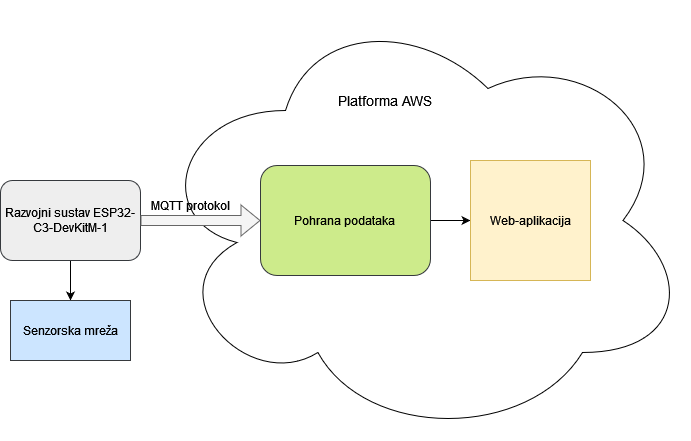
\includegraphics[width=\linewidth]{imgs/shema}
	\caption{Blok shema sustava}
	\label{fig:shema}
\end{figure}


\chapter{Razvojni sustav ESP32-C3-DevKitM-1}

Razvojni sustav temelji se na modulu ESP32-C3-MINI-1. Modul je jedan u nizu ESP32-­C3 serije SoC \engl{System on Chip} platformi tvrtke \textit{Espressif}, te sadrži jednojezgreni 32-bitni procesor s RISC-V arhitekturom koji radi na frekvenciji do 160 MHz. Modul sadrži 400 KB memorije tipa SRAM \engl{Static random-access memory}, od kojih je 16 KB rezervirano za priručnu memoriju \engl{cache}, 384 KB memorije tipa ROM \engl{Read-only memory} te 4 MB memorije tipa \textit{Flash}. Od periferije sadrži 22 programabilna GPIO pina \engl{General Purpose Input Output}, te digitalna sučelja SPI, UART, I2C i I2S. Također sadrži upravljače za sučelja USB i JTAG koji se mogu koristiti za efikasnije otklanjanje pogrešaka u kodu \engl{debugging}. Konfiguracija sustava prikazana je na slici \ref{fig:esp32}. \cite{esp32manual}

\begin{figure}[ht]
	\centering
	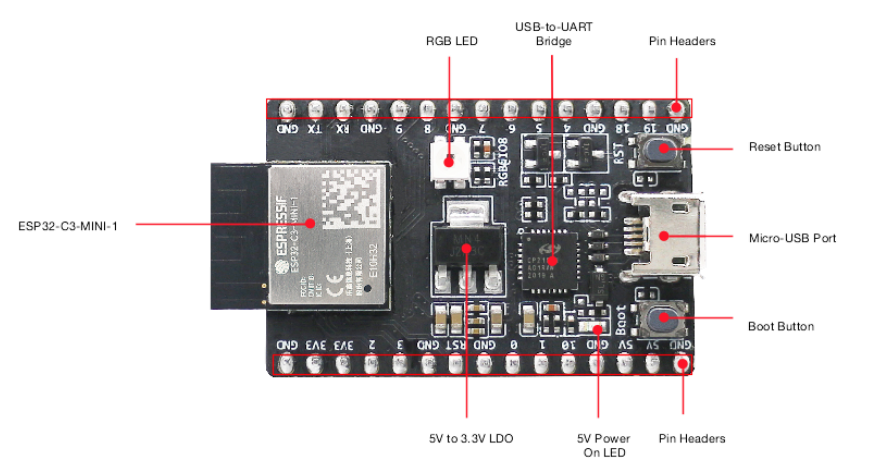
\includegraphics[scale=0.6]{imgs/esp32}
	\caption{Konfiguracija razvojnog sustava ESP32-C3-DevKitM-1 \cite{espressif}}
	\label{fig:esp32}
\end{figure}

Budući da modul ima funkciju RF \engl{radio frequency} primopredajnika, podržava bežično lokalno umrežavanje odnosno Wi-Fi, koji omogućava propusnost do 20 Mbps protokolom TCP te maksimalnu propusnost od 30 Mbps koristeći protokol UDP. Isto tako, podržava protokol Bluetooth s podrškom za velike udaljenosti. 

Modul ESP32-C3-MINI-1 bežični je uređaj niske potrošnje energije \engl{ultra-low-power} primarno namijenjen razvoju aplikacija koje koriste Wi-Fi ili \textit{Bluetooth Low Energy} (BLE) protokol. Na slici \ref{fig:esp32block} nalazi se blok shema modula sa svim dostupnim značajkama. 

\begin{figure}[ht]
	\centering
	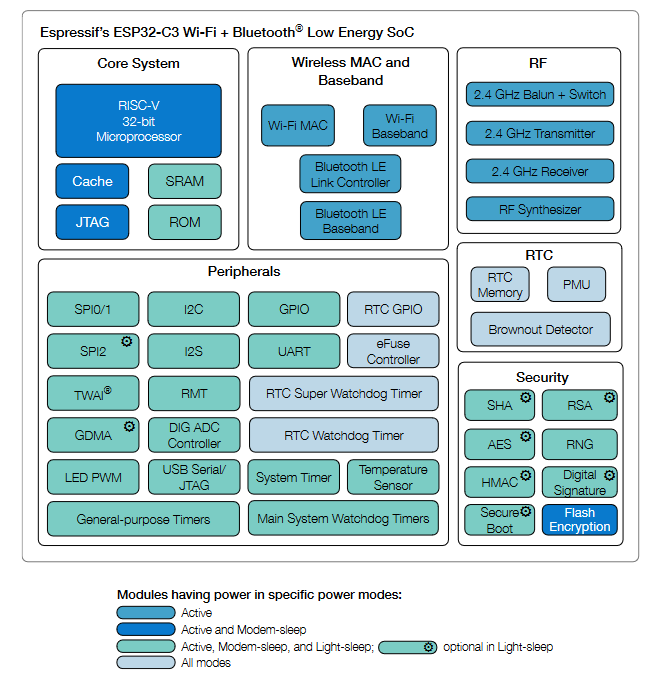
\includegraphics[scale=0.6]{imgs/esp32block}
	\caption{Blok dijagram modula ESP32-C3 \cite{esp32manual}}
	\label{fig:esp32block}
\end{figure}

IEEE 802.11, skupina standarda za bežične lokalne mreže \engl{WLANs} \cite{ieee}, nudi nekoliko različitih načina bežične modulacije signala. Pojedini standardi označeni su slovima abecede. Za korisničke mreže postoje dva frekvencijska pojasa: 2,4 GHz i 5 GHz. 

Prednosti pojasa od 2,4 GHz su veći doseg, bolje prolaženje kroz fizičke prepreke te bolja podrška jer više bežičnih uređaja koristi pojas od 2,4 GHz nego od 5 GHz. S druge strane, ovaj pojas ima manju propusnost i nudi manje kanala koji se ne preklapaju. Isto tako, može doći do zagušenja mreže jer kućni i Bluetooth uređaji koriste ovaj isti mrežni pojas.

Pojas od 5 GHz nudi brži protok, manje zagušenih kanala te ima više kanala koji se međusobno ne preklapaju. Ipak, ima kraći raspon u usporedbi s mrežama od 2,4 GHz jer teže prolazi kroz prepreke. \cite{microsoft_ieee} 

U nastavku su opisani ključni standardi Wi-Fi tehnologije \cite{how_wifi_works}:
\begin{itemize}
	\item 802.11b - najsporiji i najjeftiniji standard, emitira u frekvencijskom pojasu od 2,4 GHz. Može prenijeti do 11 Mbps te koristi komplementarno šifriranje \engl{complementary code keying - CCK} radi poboljšanja brzine prijenosa.
	\item 802.11a - transmitira u pojasu od 5 GHz i može prenijeti do 54 Mbps. Koristi ortogonalno frekvencijsko multipleksiranje \engl{orthogonal frequency-division multiplexing - OFDM}, što je efikasnija tehnika u odnosu na CCK koja dijeli radio signal u nekoliko podsignala prije slanja primatelju. Ova metoda značajno umanjuje interferenciju. 
	\item 802.11g - poput standarda 802.11b, koristi frekvencijski pojas od 2,4 GHz. Međutim, može prenijeti do 54 Mbps jer koristi tehniku OFDM.
	\item 802.11n - kompatibilan je standard sa prethodno opisanim standardima. Nudi znatno poboljšanje u rasponu i brzini u odnosu na svoje prethodnike. Ovaj standard može prenijeti do četiri toka podataka, svaki maksimalno 150 Mbps, no većina usmjerivača \engl{router} dopušta dva ili tri toka.
	\item 802.11ac - radi isključivo u pojasu od 5 GHz, te je kompatibilan s prethodnim standardima. Manje je sklon interferenciji i brži je od prethodnih standarda s maksimalnim prijenosom od 450 Mbps jednim tokom. 
	\item 802.11ax - najnoviji standard koji proširuje nekoliko ključnih mogućnosti svojih prethodnika. Usmjerivači koji podržavaju ovaj standard dopuštaju tok podataka do 9.2 Gbps, što je značajan porast u usporedbi s prethodnicima. Isto tako, moguće je postaviti više antena na jedan usmjerivač, čime je omogućen prihvat više veza odjednom bez usporavanja i interferencije.
\end{itemize}

Podsustav modula ESP32-C3 za Wi-Fi u skladu je sa standardom IEEE 802.111 te koristi nelicencirani pojas frekvencija od 2,4 GHz. U tom pojasu podržava propusnost od 20 i 40 MHz. Modul također podržava tehniku raznolikosti antena \engl{antenna diversity} za poboljšanje prijema i pouzdanosti signala korištenjem RF komutatora \engl{switch}. Tim komutatorom upravljaju GPIO priključci i koristi se za odabir najbolje antene u kontekstu pouzdanosti i kvalitete signala. \cite{esp_mini}

ESP32-C3 u potpunosti implementira protokol Wi-Fi na temelju standarda 802.11 b/g/n. Podržava osnovni skup \engl{Basic Service Set - BSS} operacija za značajke pristupne točke \engl{software enabled access point - SoftAP}. Ovakve pristupne točke koriste softver kako bi omogućile uređajima kojima primarna svrha nije usmjeravanje prometa da postanu virtualni usmjerivač. \cite{what_is_softap} Također, upravljanje napajanjem odvija se automatski s minimalnom intervencijom domaćina kako bi se smanjila aktivnost uređaja.

Tvrtka \textit{Espressif} također nudi biblioteke za povezivanje putem protokola TCP i IP te korištenje Wi-Fi \textit{mesh} tehnologije. Pruža i podršku za protokole TLS 1.0, 1.1 i 1.2. Na slici \ref{fig:wifi_rf_table} prikazani su Wi-Fi RF standardi koje koristi modul. 

\begin{figure}[ht]
	\centering
	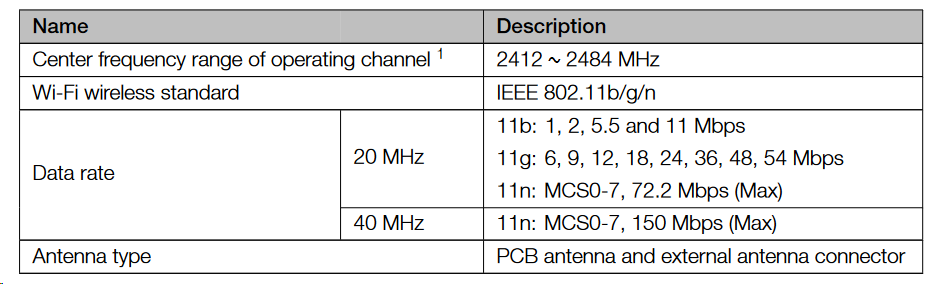
\includegraphics[scale=0.5]{imgs/wifi_rf_table}
	\caption{Wi-Fi RF standardi \cite{esp_mini}}
	\label{fig:wifi_rf_table}
\end{figure}

ESP32 nudi nekoliko načina rada pri korištenju Wi-Fi tehnologije \cite{esp_wifi_connect_overview}:
\begin{enumerate}
	\item način rada stanice \engl{station mode} - ESP32 spaja se na točku pristupa,
	\item način rada pristupne točke \engl{SoftAP mode} - druge se stanice spajaju na ESP32,
	\item miješani - ESP32 radi kao stanica i pristupna točka spojena na drugu pristupnu točku. 
\end{enumerate}

U nastavku su opisani scenariji Wi-Fi povezivanja modula ESP32-C3 u načinu rada stanice i pristupne točke.

Na slici \ref{fig:station_scenario} prikazan je sekvencijski dijagram zadataka koje ESP32 obavlja u cijelom ciklusu spajanja i komunikacije s pristupnom točkom. Iz slike je vidljivo da se ciklus sastoji od osam faza. Prva faza služi za inicijalizaciju upravljačkih programa i pokretanje zadataka odnosno dretvi koje će obavljati zadatke vezane uz svoju dužnost. Glavni zadatak pokreće četiri različite dretve izvršavanja: aplikacijski zadatak, zadatak za događaje, zadatak za IP protokol, te zadatak za Wi-Fi. U drugoj fazi konfigurira se upravljački program za Wi-Fi. U sljedećoj se fazi pokreće upravljački program, nakon koje slijedi faza pretraživanja mreže i povezivanja na usmjerivač ili pristupnu točku. Nakon inicijalizacije DHCP klijenta, započinje faza dohvata IP adrese. Šesta faza odvija se nakon prekida Wi-Fi veze, čime se također uklanjaju i sve UDP i TCP konekcije. U aplikaciji se može omogućiti radno čekanje na ponovno uspostavljanje veze. Sedma faza pokreće se pri detekciji promjene IP adrese. Posljednja faza služi za programsko odspajanje s mreže i zaustavljanje upravljačkog programa za Wi-Fi.

Slika \ref{fig:ap_scenario} modelira slučaj u kojem ESP32 ima ulogu pristupne točke. Scenarij je vrlo sličan ranije opisanom slijedu događaja, no razlikuje se u dvije faze i događajima koji su pohranjeni u sustavu. Ovaj način rada nema fazu detekcije promjene IP adrese, jer je u ovom načinu ESP32 upravo taj uređaj čija se IP adresa može promijeniti. Isto tako, ne postoji faza dohvata IP adrese. 

\begin{figure}[ht]
	\centering
	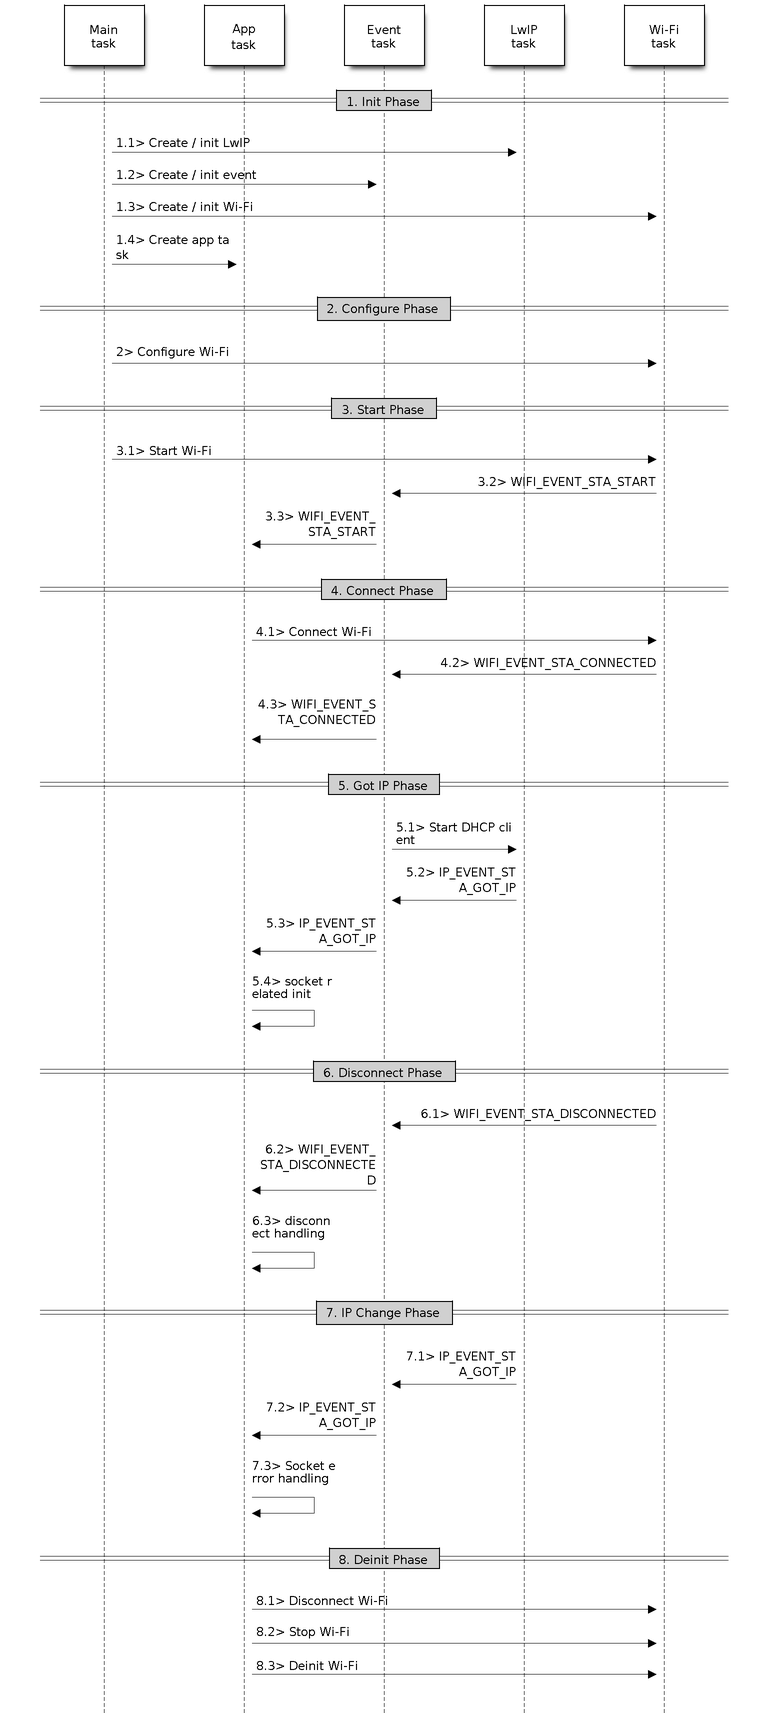
\includegraphics[scale=0.3]{imgs/station_scenario}
	\caption{Primjer scenarija Wi-Fi povezivanja u načinu rada stanice \cite{espressif}}
	\label{fig:station_scenario}
\end{figure}

\begin{figure}[ht]
	\centering
	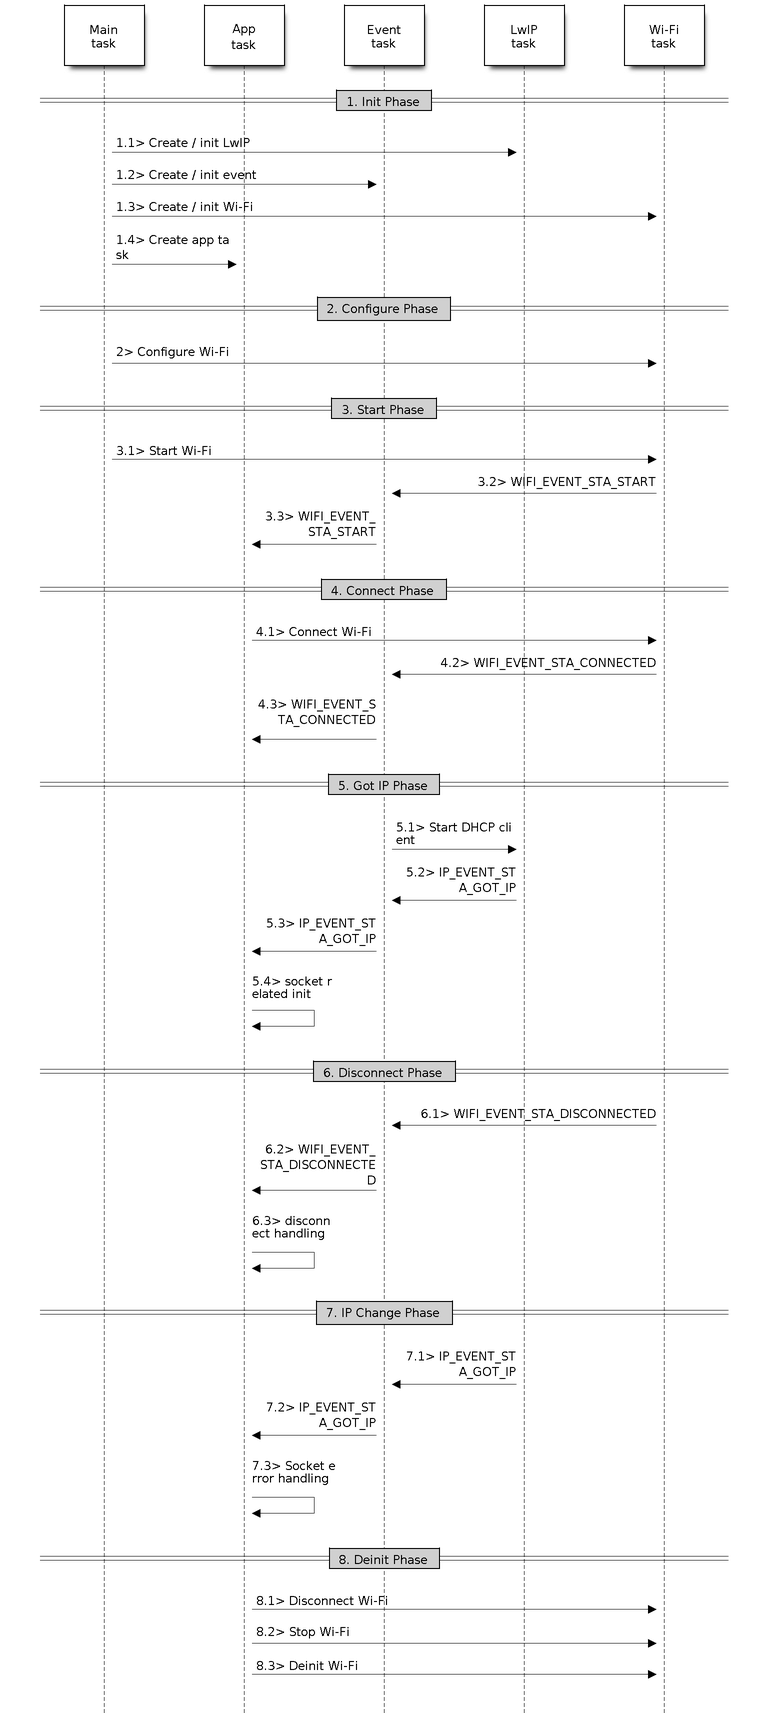
\includegraphics[scale=0.3]{imgs/station_scenario}
	\caption{Primjer scenarija Wi-Fi povezivanja u načinu rada pristupne točke \cite{espressif}}
	\label{fig:ap_scenario}
\end{figure}

U modulu ESP32 stavljen je veliki naglasak na mehanizme uštede energije, što se također preslikava na korištenje Wi-Fi veze. Modul pruža načine uštede energije i pri radu kao stanica i pristupna točka, no neke značajke nisu podržane u pristupnoj točki. Modul pri neaktivnosti može otići u stanje mirovanja \engl{sleep mode}. Postoje dva načina uštede energije u načinu rada stanice: minimalna i maksimalna ušteda. Pri minimalnoj uštedi stanica se budi iz stanja mirovanja nakon svakog DTIM intervala \engl{Delivery Traffic Indication Message}. Ovim se načinom ne gube globalno emitirane poruke \engl{broadcast} jer se one prenose nakon DTIM intervala. Međutim, ova metoda ne štedi puno energije ako je pristupna točka na koju je spojen modul postavila malen interval. Pri maksimalnoj uštedi moguće je znatno produžiti vrijeme mirovanja u odnosu na DTIM interval, no ovime se riskira gubitak globalno emitiranih poruka. 

\eject
\chapter{Amazon Web Services (AWS)}

Amazon usluge za web \engl{Amazon Web Services - AWS} sveobuhvatna je platforma za računarstvo u oblaku koju pruža tvrtka Amazon te sadrži brojne usluge u oblaku, uključujući infrastrukturu \engl{Infrastructure as a Service - IaaS}, platformu \engl{Platform as a Service - PaaS} i softver \engl{Software as a Service - SaaS}. AWS usluge nude organizacijske alate kao što su računalna snaga, baza podataka i usluge isporuke sadržaja \cite{what_is_aws}. 

AWS je podijeljen u više različitih usluga koje se mogu pojedinačno konfigurirati na temelju korisničkih potreba. Neke od usluga koje nudi AWS su: pohrana, baze podataka, monitoriranje, sigurnost, analitika, umjetna inteligencija te razvoj mobilnih aplikacija. 

AWS pruža usluge iz mnogo podatkovnih centara \engl{data center - DC} koji su raspodijeljeni po zonama dostupnosti \engl{availability zone - AZ} diljem regija cijelog svijeta. Jedna regija obuhvaća nekoliko fizički bliskih zona povezanih mrežom niske latencije. Geografskom raspodijeljenošću AWS pruža višestruke prednosti \cite{aws_regions}:
\begin{enumerate}
	\item niska latencija: budući da su regije skupovi fizičkih mrežno povezanih bliskih zona, korisnički podaci i aplikacije mogu biti smješteni bliže krajnjim korisnicima što poboljšava performanse aplikacija,
	\item visoka dostupnost: u slučaju kvara podatkovnog centra, korištenjem više zona dostupnosti unutar regije podaci mogu i dalje ostati dostupni,
	\item otpornost i oporavak od katastrofe: podaci i aplikacije mogu se replicirati između više zona ili regija, što omogućava brzi oporavak u slučaju prirodnih katastrofa, tehničkih problema ili napada,
	\item skalabilnost: klijenti mogu dinamički povećavati ili smanjivati resurse u različitim regijama ovisno o potražnji,
	\item poboljšana sigurnost: fizički odvojeni podatkovni centri smanjuju rizik od pojedinačnih točaka neuspjeha i omogućavaju implementaciju složenijih sigurnosnih strategija.
\end{enumerate}

Također, nude se brojne mogućnosti za razvojne inženjere u sklopu AWS-a. Nudi alate naredbenog retka \engl{command-line tools} i pakete za razvoj programa \engl{Software Development Kit - SDK} za puštanje aplikacija u produkciju \engl{deployment} i upravljanje vlastitim uslugama i aplikacijama. Paketi za razvoj programa dostupni su u raznim programskim jezicima, uključujući programske jezike C++, Android, iOS, Java, Node.js, Python i Ruby.

AWS isto tako nudi brojne usluge za razvoj IoT sustava. Usluga AWS-a za IoT pruža platformu za upravljanje IoT uređajima te obradu podataka i njihovu pohranu na druge AWS usluge, poput baze podataka. AWS IoT pruža usluge u oblaku koje povezuju IoT uređaje s drugim uređajima i uslugama AWS-a u oblaku. Također pruža softver za uređaje, poput paketa za razvoj programa, za jednostavniju integraciju s uslugama AWS-a za IoT. Na slici \ref{fig:aws_iot_arch} nalazi se prikaz arhitekture usluga koje AWS nudi za razvoj IoT sustava.

\begin{figure}[ht]
	\centering
	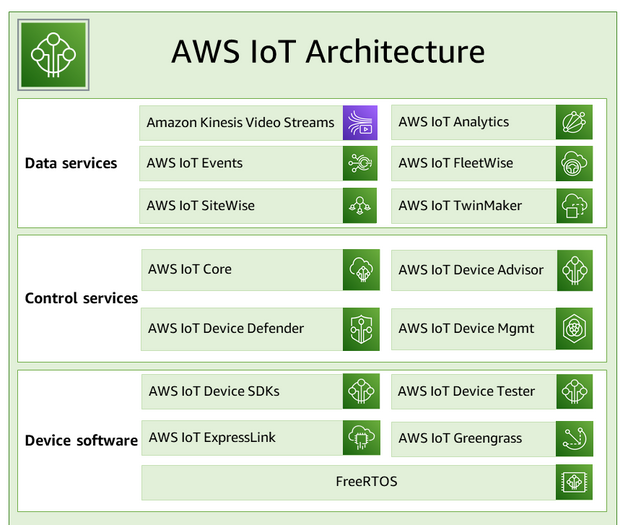
\includegraphics[scale=0.8]{imgs/aws_iot_arch}
	\caption{Arhitektura usluga AWS-a za IoT \cite{aws_docs}}
	\label{fig:aws_iot_arch}
\end{figure}

AWS podržava sljedeće komunikacijske protokole za IoT sustave:
\begin{itemize}
	\item MQTT \engl{Message Queuing Telemetry Transport},
	\item HTTPS,
	\item LoRaWAN \engl{Long Range Wide Area Network},
	\item TLS.
\end{itemize}

U nastavku su opisane usluge koje nudi AWS za razvoj IoT sustava.

\section{AWS IoT Core}

AWS IoT Core ključna je komponenta za integraciju oblaka i fizičkih uređaja. Omogućava povezivanje uređaja i preusmjeravanje poruka na usluge AWS-a. Koristi MQTT koji je standardni protokol za razmjenu poruka u IoT sustavima. To je lagan \engl{lightweight} protokol za prijenos poruka temeljen na objavi/pretplati sustavu u kojoj glavnu ulogu ima broker kao posrednik, te je pogodan za povezivanje udaljenih uređaja uz minimalnu potrošnju \cite{what_is_mqtt}. AWS IoT Core pruža paletu značajki za razmjenu poruka temeljenih na protokolu MQTT, koje pomažu pri izradi prilagodljive i skalabilne IoT arhitekture \cite{aws_docs}. Komponenta također ima ugrađenu podršku za upravljanje MQTT brokerom koji podržava trajne, uvijek uključene veze, napredna pravila zadržavanja poruka te obrađuje više uređaja i tema istovremeno. Isto tako, AWS IoT Core podržava najnoviji standard MQTT 5 i kompatibilan je sa prethodnim standardom MQTT 3, što omogućuje učinkovito upravljanje heterogenim implementacijama s mnoštvom specifikacija. Nadalje, komponenta omogućava višestruke metode provjere autentičnosti i pristupne politike za zaštitu rješenja od ranjivosti. Štoviše, koristeći pomoć drugih usluga u sklopu platforme kao što je AWS IoT Core Device Advisor, moguće je pristupiti unaprijed izgrađenim paketima testova za provjeru MQTT funkcionalnosti uređaja tijekom faze razvoja.

Na slici \ref{fig:aws_iot_core_overview} nalazi se pregled rada usluge AWS IoT Core.

\begin{figure}[ht]
	\centering
	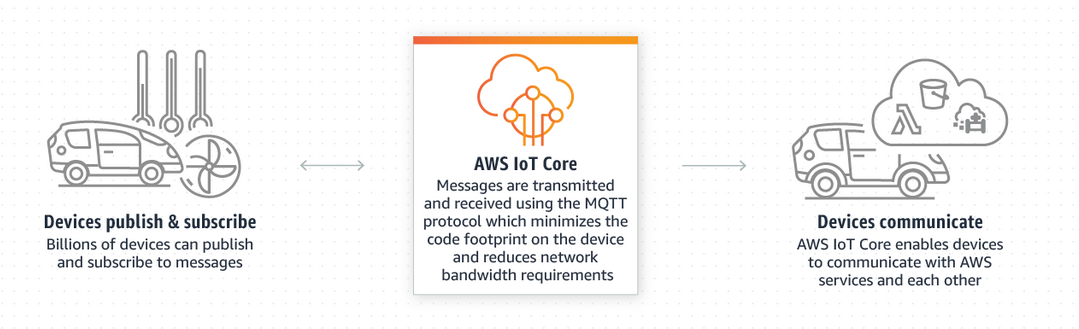
\includegraphics[scale=0.6]{imgs/aws_iot_core_overview}
	\caption{Princip rada usluge AWS IoT Core \cite{aws_docs}}
	\label{fig:aws_iot_core_overview}
\end{figure}

AWS IoT Core pruža usluge koje povezuju oblak AWS-a s IoT uređajima kako bi se ostale usluge u oblaku i aplikacije mogle međusobno komunicirati s tim uređajima. Na slici \ref{fig:aws_iot_core_components} nalaze se svi segmenti usluge AWS IoT Core te kako oni komuniciraju s vanjskim dijelovima. Zelenom bojom označena je sama usluga, narančastom bojom fizički uređaji odnosno stvari (engl. \textit{Things}), sivom bojom druge IoT aplikacije unutar AWS-a koje se mogu izravno spojiti na sustave u AWS-u, dok su plavom bojom označene ostale usluge odnosno sustavi koji se nalaze u ekosustavu AWS.

\begin{figure}[ht]
	\centering
	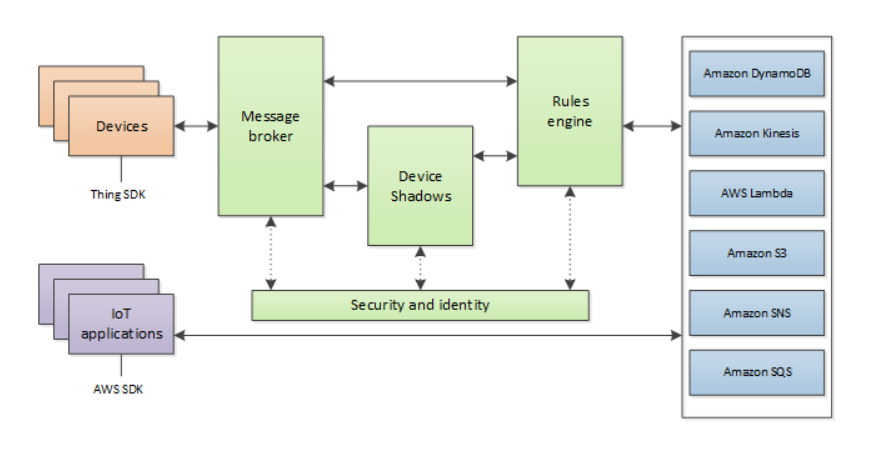
\includegraphics[scale=0.6]{imgs/aws_iot_core_components}
	\caption{Komponente usluge AWS IoT Core \cite{aws_docs}}
	\label{fig:aws_iot_core_components}
\end{figure}

U nastavku su ukratko opisane ključne usluge koje pokriva AWS IoT Core \cite{aws_docs}.

\subsubsection{Usluge za slanje poruka}

AWS IoT Core usluge za povezivanje pružaju sigurnu komunikaciju s IoT uređajima i upravlja porukama koje prolaze između uređaja i oblaka.

Prilazni uređaj omogućuje uređajima sigurnu i efikasnu komunikaciju sa sustavom AWS. Komunikacija je osigurana sigurnosnim protokolima koji koriste  X.509 certifikate. 

Broker za poruke pruža mehanizam uređajima i aplikacijama slanje i primanje poruka. Moguće je koristiti protokol MQTT ili direktno \textit{WebSocket} za objavu i pretplatu na teme. Uređaji i klijenti koriste sučelje HTTP REST za objavu poruka brokeru. Broker zatim distribuira podatke na uređaje koji su se pretplatili na određene teme kao i na druge AWS aplikacije te usluge koje prate teme na brokeru.

AWS IoT Core za protokol LoRaWAN omogućava postavljanje privatne LoRaWAN mreže tako što poveže LoRaWAN te prilazne uređaje na AWS bez potrebe za razvojem mrežnog servera za LoRaWAN \engl{LoRaWAN Network Server - LNS}. Poruke primljene od LoRaWAN uređaja šalju se na stroj za pravila \engl{rules engine} gdje se formatiraju i prosljeđuju ostalim AWS uslugama.

Stroj za pravila \engl{rules engine} povezuje podatke iz brokera s drugim AWS IoT uslugama za pohranu i dodatnu obradu. Primjerice, moguće je umetati ili pretraživati po podatkovnim tablicama ili pozvati određene definirane funkcije na temelju izraza definiranog u stroju. Isto tako, moguće je obraditi te podatke i proslijediti novostvoreni format poruka drugim uslugama ili bazama podataka.

\subsubsection{Upravljačke usluge}

Upravljačke usluge AWS IoT Core komponente pružaju sigurnost uređaja te značajke za upravljanje i registraciju novih uređaja.

Moguće je definirati vlastite autorizatore radi upravljanja autentifikacijskim i autorizacijskim strategijama koristeći vlastiti servis za autentifikaciju i funkcije za računanje Lambda koje nudi AWS. Lambda je računalna usluga za slučajeve i aplikacije dinamičke skalabilnosti. Pokreće kod na infrastrukturi visoke dostupnosti i obavlja cjelokupnu administraciju računalnih resursa, uključujući održavanje poslužitelja i operativnog sustava, osiguravanje kapaciteta i automatsko skaliranje ovisno o trenutnim potrebama sustava. Lambda funkcije korisne su za obradu datoteka, tokova te HTTP zahtjeva. Funkcije su pogodne za obradu podataka prije preusmjeravanja na drugu funkciju ili pohranu. 

Usluga za registraciju uređaja u sustav \engl{provisioning} omogućava konfiguriranje i prijavu uređaja u AWS koristeći predložak koji opisuje resurse potrebne uređaju: stvar, certifikat i nekoliko politika. Stvar \engl{thing} je unos u registar koji sadrži atribute opisa uređaja. Uređaji koriste certifikate za autentifikaciju sa sustavom AWS. Politike određuju koje operacije uređaj može izvršiti. Svaka politika ima definirani dokument s izjavom koja se sastoji od učinka, akcije i resursa nad kojim se akcija izvršava. Učinak može biti \textit{Dopusti} ili \textit{Uskrati}, akcija se odnosi nad radnje s MQTT brokerom i poslovima, a resurs se odnosi na regiju i račun u kojem politika vrijedi. 

Isto tako, moguće je definirati grupe za lakšu kategorizaciju i upravljanje uređajima. Grupe također mogu imati podgrupe, i tako graditi hijerarhiju grupa. Sve akcije izvršene na roditeljima propagiraju se do najdubljih podgrupa. Dozvole dodijeljene grupi primjenjuju se na sve uređaje u toj grupi i svim njihovim podgrupama. 

Usluga za poslove \engl{jobs} omogućava definiranje udaljenih operacija koje se pošalju i izvrše na fizičkim uređajima spojenih u oblak. Posao se može odnositi preuzimanje i instalaciju aplikacija, ažuriranje sustava, ponovno pokretanje, obnova certifikata i slično.

Usluga za sigurnost i identitet pruža dijeljenu odgovornost za sigurnost unutar AWS oblaka. Fizički uređaji moraju držati vjerodajnice na sigurnom kako bi se podaci mogli slati brokeru na siguran način. Značajke za sigurnost koriste i stroj za pravila kao i broker za poruke radi sigurnog prijenosa podataka drugim uslugama unutar AWS ekosustava.

\subsubsection{Usluge za uređaje}

AWS IoT Core osigurava pouzdano aplikacijsko iskustvo iako uređaji nisu uvijek povezani. 

Sjena uređaja \engl{Device Shadow} dokument je u JSON formatu koji se koristi za pohranu i dohvat trenutnog stanja i informacija o uređaju. AWS nudi uslugu koja održava stanje uređaja \engl{Device Shadow service} kako bi aplikacije mogle komunicirati s uređajem bez obzira je li uređaj na mreži ili ne. Kada uređaj nije priključen na mrežu, usluga sjene uređaja upravlja podacima za povezane uređaje. Kada se uređaj ponovno spoji na mrežu, sinkronizira stanje sa sjenom uređaja koja se nalazi u oblaku. Uređaji također mogu objavi svoje stanje usluzi u bilo kojem trenutku kako bi bilo na raspolaganju drugim aplikacijama i uređajima. 

\subsection{AWS IoT Fleet Provisioning}

Kao što je ranije navedeno, AWS nudi uslugu registracije uređaja u sustav čime uređaj dobiva pristup ostalim uslugama unutar platforme, poput povezivanja na MQTT broker. Moguće je dinamički registrirati više uređaja pomoću privremenih ili trajnih certifikata, što se naziva provizioniranje flote \engl{fleet provisioning}. Pomoću ove usluge AWS generira i sigurno dostavi certifikate te privatne ključeve na uređaje pri prvom povezivanju na platformu. AWS izdaje klijentske certifikate koji su potpisani certifikacijskim tijelom tvrtke Amazon \engl{Certificate Authority - CA} \cite{aws_docs}.

Tri su ključna koraka pri omogućavanju registracije više uređaja u sustav:
\begin{enumerate}
	\item određivanje načina registracije,
	\item definiranje upravljačke strukture nad uređajima,
	\item kreiranje predloška za registraciju.
\end{enumerate}

Određivanje načina registracije u sustav povezano je s odabirom vrste certificiranja koja će se koristiti. Uređaji trebaju jedinstveni certifikat za povezivanje s platformom AWS i korištenje njenih usluga. Postoje tri metode certificiranja uređaja te odabir ovisi o mogućnostima proizvodnje uređaja i ovlastima samih korisnika:
\begin{itemize}
	\item registracija uređaja vlastitim jedinstvenim certifikatima, 
	\item registracija od strane korisnika od povjerenja,
	\item registracija certifikatom zahtjeva.  
\end{itemize} 

Registracija uređaja vlastitim jedinstvenim certifikatima podrazumijeva postojanje verificiranih certifikata na samom uređaju pri prvom povezivanju u sustav. Ovaj se način još naziva i pravodobno provizioniranje \engl{just-in-time provisioning}. Problem s ovim pristupom jest što instalacija certifikata nije uvijek moguća prije dostave uređaja korisniku. Isto tako, čak iako je instalacija certifikata moguća, nije uvijek moguće instalirati certifikate sigurno na uređaj, stoga je potrebno koristiti alternativne metode. 

U slučaju kada rana certifikacija uređaja nije moguća, autorizirani ili krajnji korisnici \engl{trusted users} mogu uz pomoć aplikacije registrirati uređaje prije njihova spajanja na platformu. Ovdje je potrebno korisnicima pružiti aplikaciju kojom bi konfigurirali uređaj prilikom instalacije, te \textit{firmware} uređaja mora podržavati ovaj način registracije. 

Treća opcija jest registracija pomoću certifikata zahtjeva \engl{claim certificate}. Certifikati zahtjeva privremeni su certifikati koji se mogu instalirati na više uređaja, te se pri prvoj registraciji u sustav zamijene s novim, jedinstvenim certifikatom. Ova metoda zahtijeva dodatne sigurnosne provjere zbog mogućnosti curenja privremenih certifikata zahtjeva jer više uređaja dijeli isti certifikat, no prijetnja se može ublažiti redovitim rotiranjem privremenih certifikata te kreiranjem više certifikata zahtjeva koji se mogu koristiti. Isto tako, privremenim certifikatima potrebno je dodijeliti minimalan skup dozvoljenih radnji potrebnih za registraciju uređaja. Dodatna sigurnosna provjera može se izvršiti i u obliku Lambda funkcije dodatnom provjerom primljenih parametara s uređaja.

Upravljačka struktura nad uređajima je važna radi lakše organizacije uređaja u samom sustavu. Povezani uređaji predstavljeni su u platformi kao stvari tj. resursi koji se mogu organizirati i održavati. Osim ranije spomenutih stvari i grupa stvari, moguće je uređajima dodijeliti atribute po kojima se može pretraživati. Atributi se isto tako mogu dinamički dodijeliti na temelju podataka s uređaja prilikom njegove registracije. Oni se definiraju u predlošku za registraciju. 

Predložak za registraciju dokument je u formatu JSON koji opisuje resurse, politike i dozvole koje je potrebno dodijeliti uređaju kada je registriran. Odjeljak \textit{parametri} u predlošku definira resurse u odjeljku \textit{resursi} koje uređaj mora koristiti pri interakciji s platformom. Svaki parametar definira naziv, vrstu i zadanu vrijednost koja nije obavezna. Zadana vrijednost koristi se kada rječnik proslijeđen s predloškom ne sadrži vrijednost za parametar. Odjeljak \textit{parametri} izgleda na sljedeći način:

\begin{lstlisting}[caption={Odjeljak \textit{parametri} u predlošku za registraciju}, language=json]
	{
		"Parameters" : {
			"ThingName" : {
				"Type" : "String"
			},
			"SerialNumber" : {
				"Type" : "String"
			},
			"Location" : {
				"Type" : "String",
				"Default" : "HR"
			},
			"CSR" : {
				"Type" : "String"    
			}
		}
	}
\end{lstlisting}

Odjeljak \textit{resursi} u predlošku definira resurse koji su potrebni uređaju za daljnji rad i komunikaciju sa sustavom: stvar, certifikat, jedna ili više politika. Svaki resurs specificira naziv, vrstu i skup svojstava. Vrsta resursa može biti jedna od tri vrijednosti: \lstinline|AWS::IoT::Thing|, \lstinline|AWS::IoT::Certificate|, te \lstinline|AWS::IoT::Policy|. Resursi tipa certifikat imaju posebna svojstva koja ih definiraju, ovisno o tome koja je metoda registracije uređaja odabrana. Politike su vezane za već postojeće politike u sustavu AWS. Odjeljak \textit{resursi} može izgledati na sljedeći način:

\begin{lstlisting}[caption={Odjeljak \textit{resursi} u predlošku za registraciju}, language=json]
{ 
	"Resources" : {
		"thing" : {
			"Type" : "AWS::IoT::Thing",
			"Properties" : {
				"ThingName" : {"Ref" : "ThingName"},
				"AttributePayload" : { "version" : "v1", "serialNumber" :  {"Ref" : "SerialNumber"}}, 
				"ThingTypeName" :  "lightBulb-versionA",
				"ThingGroups" : ["v1-lightbulbs", {"Ref" : "Location"}]
			},
			"OverrideSettings" : {
				"AttributePayload" : "MERGE",
				"ThingTypeName" : "REPLACE",
				"ThingGroups" : "DO_NOTHING"
			}
		},  
		"certificate" : {
			"Type" : "AWS::IoT::Certificate",
			"Properties" : {
				"CertificateSigningRequest": {"Ref" : "CSR"},
				"Status" : "ACTIVE"      
			}
		},
		"policy" : {
			"Type" : "AWS::IoT::Policy",
			"Properties" : {
				"PolicyDocument" : "{ \"Version\": \"2012-10-17\", \"Statement\": [{ \"Effect\": \"Allow\", \"Action\":[\"iot:Publish\"], \"Resource\": [\"arn:aws:iot:us-east-1:123456789012:topic/foo/bar\"] }] }"
			}
		}
	}
}
\end{lstlisting}

Valja napomenuti kako je moguće u korisničkom sučelju platforme odabrati sve parametre, te kreiranje vlastitog dokumenta u JSON formatu nije potrebno, nego se automatski generira iz korisničkog odabira u sučelju. 

\subsection{AWS IoT Device Shadow}

Usluga sjene uređaja \engl{Device Shadow} omogućava održavanje trenutnog stanja uređaja, čak i kada su uređaji privremeno nedostupni. AWS nudi uslugu koja održava stanje uređaja kako bi aplikacije mogle komunicirati s uređajem bez obzira je li uređaj na mreži ili ne. Kada uređaj nije priključen na mrežu, usluga sjene uređaja upravlja podacima za povezane uređaje. Kada se uređaj ponovno spoji na mrežu, sinkronizira stanje sa sjenom uređaja koja se nalazi u oblaku. Uređaji također mogu objaviti svoje stanje usluzi u bilo kojem trenutku kako bi bilo na raspolaganju drugim aplikacijama i uređajima. Ova funkcionalnost ključna je za slučajeve u kojima uređaji nemaju konstantnu povezanost na mrežu ili rade u udaljenim ili nepouzdanim mrežnim uvjetima.

\subsection{AWS IoT Jobs}

Pokretanje poslova u sklopu usluge AWS IoT Jobs, kao što je ranije spomenuto, služi za udaljene operacije na fizičkim uređajima povezanih s platformom. 

Posao je udaljena operacija koja se šalje i izvodi na jednom ili više uređaja povezanih s uslugom AWS IoT. Primjerice, moguće je definirati posao koji upućuje skup uređaja da preuzmu i instaliraju aplikaciju ili pokreću ažuriranja, rotiraju certifikate te je moguće udaljeno rješavati nastale probleme na uređajima \engl{remote troubleshooting}. Da bi se kreirao posao, najprije je potrebno kreirati dokument posla \engl{job document} koji je opis udaljenih operacija koje će uređaji izvesti. Dokumenti posla sadrže informacije koje su potrebne uređajima za obavljanje posla te su u formatu JSON. Dokumenti se mogu pohraniti na platformu i posebno dohvaćati, no isto tako mogu se definirati uz samu naredbu koja izvršava posao. Pri kreiranju posla, potrebno je specificirati odredišne uređaje \engl{targets} koji trebaju izvršiti naredbe. Moguće je odabrati pojedinačne uređaje, ali i grupu uređaja. Usluga zatim pošalje poruku svakom uređaju da postoji posao dostupan za izvršavanje. Nakon kreiranja posla, dokument posla se postavlja na udaljene uređaje koje je potrebno ažurirati. Ciljni uređaj preuzima taj certifikat i time započinje izvršavanje posla. Izvodi operacije opisane u dokumentu i o napretku obavještava platformu. Broj izvršenja \engl{execution number} jedinstveni je identifikator izvršenja posla na određenom ciljnom uređaju. Usluga izvršavanja posla pruža naredbe za praćenje napretka izvršenja posla na uređaju kao i na svim uređajima. 

Na temelju broja ponavljanja posla, razlikuju se dvije vrste poslova:
\begin{enumerate}
	\item jednokratni posao \engl{snapshot job}: posao se šalje svim odabranim ciljnim uređajima pri kreiranju posla, te nakon odrađivanja posla ili odgovora o nemogućnosti izvršenja, posao se smatra gotovim, 
	\item kontinuirani posao \engl{continuous job}: definiran je na razini grupe stvari, te se pri dodavanjem svakog novog uređaja u grupu izvršava na dodanom uređaju. 
\end{enumerate}

Preporučljivo je poslove označiti kontinuiranima jer se tako omogućava izvršavanje posla na novododanim uređajima čak i nakon kreiranja posla. 

Moguće je odrediti koliko se brzo ciljni uređaji obavještavaju o zakazanom izvršenju posla. To omogućuje stvaranje postupnog uvođenja \engl{staged rollout} radi boljeg upravljanja ažuriranjima, ponovnim pokretanjem i drugim operacijama. Konfiguraciju uvođenja moguće je izraditi koristeći statičku ili eksponencijalnu stopu uvođenja. Za navođenje maksimalnog broja uređaja koji se mogu obavijestiti u minuti, potrebno je koristiti statičku stopu. 

Raspored poslova omogućuje raspoređivanje vremenskog okvira uvođenja dokumenta posla na sve ciljne uređaje. Osim toga, moguće je stvoriti vremenski okvir održavanja sa specifičnim datumima i vremenima unutar kojeg se dokument posla šalje na sve uređaje. Taj se vremenski okvir održavanja provodi na proizvoljnoj vremenskoj bazi, primjerice tjedno, ili pak na određene prilagođene datume koji se odaberu pri inicijalnom postavljanju posla. Samo se kontinuirani poslovi mogu izvršavati periodički tokom održavanja budući da se oni mogu ponavljati. Maksimalno trajanje ponavljajućeg vremenskog okvira održavanja je 23 sata i 50 minuta. Jednokratni poslovi također se mogu uvrstiti u raspored poslova, no njima nije omogućeno izvršavanje unutar vremenskog okvira održavanja, nego jednokratno u definiranom vremenskom trenutku. 

Za zakazane poslove koji se izvršavaju tijekom prozora održavanja s ručno postavljenom učestalošću izvršavanja, učestalost odnosno frekvencija definira se izrazom u formatu posla \textit{cron}. U operacijskim sustavima tipa \textit{Unix}, posao tipa \textit{cron} jest zadatak koji se kreira pomoću alata \textit{cron}, što je alat za zakazivanje i automatizaciju budućih poslova \cite{cron}. Pomoću njih automatizira se održavanje sustava, nadziranje diska, kao i pravljenje sigurnosnih kopija. Poslovi tipa \textit{cron} imaju određenu sintaksu i strukturu koja omogućava da se izvršavanje skripti pravilno izvršava. Sintaksa tipa \textit{cron} sastoji se od pet obaveznih polja međusobno odvojenih razmakom. Tablica \ref{table:cron} prikazuje polja koja se moraju definirati. 

\begin{table}[ht!]
	\centering
	\caption{Polja formata tipa \textit{cron} \cite{aws_docs}}
	\begin{tabular}{|c| c| c|}
		\hline
		\rowcolor{lightblue}  
		\textbf{Polje} & \textbf{Vrijednosti} & \textbf{Zamjenski znakovi} \\ \hline
		Minuta & 0-59 & , - * / \\ \hline
		Sat & 0-23 & , - * / \\ \hline
		Dan u mjesecu & 1-31 & , - * ? / L W \\ \hline
		Mjesec & 1-12 ili \textit{JAN-DEC} & , - * / \\ \hline
		Dan u tjednu & 1-7 ili \textit{MON-SUN} & , - * ? L \# \\ \hline
	\end{tabular}
	\label{table:cron}
\end{table}

U tablici se isto tako nalazi stupac za zamjenske znakove. Zamjenski znakovi \engl{wildcards} služe upravo kao zamjena sa konkretnu vrijednost za ona polja čija vrijednost nije bitna u kontekstu izraza. Zarez se koristi za odvajanje više vrijednosti, crtica označava opseg od prve do posljednje definirane vrijednosti, a zvjezdica je zamjena za sve vrijednosti polja. Kosa crta označava pojedinačne inkremente, a upitnik navodi jedno ili drugo. Slovo \textit{L} označava posljednji dan u tjednu ili mjesecu, a \textit{W} radni dan. Ljestve specificiraju pojedinačnu instancu unutar mjeseca, primjerice svaki drugi ponedjeljak u mjesecu. U nastavku je primjer posla u formatu \textit{cron} koji se pokreće svake minute između 15:00 i 15:59, svaki drugi dan u mjesecu, no samo siječnju i veljači:

\begin{lstlisting}[caption={Primjer formata tipa \textit{cron}}]
// min hr day month weekday
	* 15 2-30/2 JAN,FEB *
\end{lstlisting}

Moguće je postaviti otkazivanje uvođenja posla na temelju postavljenih kriterija. Poslovi se mogu otkazati ako je previše uređaja vratilo negativnu potvrdu o izvršenju posla, ili pak previše uređaja nije poslalo nikakav odgovor do isteka određenog vremenskog perioda. 

Pri isteku vremena \engl{timeout} za posao šalje se obavijest pri neočekivano dugom stanju uređaja bez ažuriranja promjene. Postoje dvije vrste mjerača vremena: aktivni mjerači \engl{in-progress timers} te mjerači koraka \engl{step timers}. Aktivni mjerači vremena ne mogu se izmijeniti nakon njihova pokretanja, te služe za mjerenje vremena izvođenja trenutno aktivnih poslova i postavljanje statusa izvršenja posla. Isto tako, ovaj mjerač vremena vrijedi za sva izvršenja istog posla, bez obzira na uređaj. Ako je potrebno pratiti odnosno ažurirati samo jedno izvršenje posla, onda se koristi mjerač koraka. On nema utjecaja na aktivni mjerač vremena. Moguće je postaviti novu vrijednost mjerača koraka pri svakom ažuriranju izvršenja posla, odnosno mjeriti trajanje svakog koraka pri izvršenju posla. 

Isto tako, moguće je pokrenuti ponovni pokušaj izvršenja posla kada posao ne uspije ili pak istekne maksimalno vrijeme izvršavanja posla. Moguće je imati najviše deset ponovnih pokušaja za izvršenje posla te se svaka iteracija može nadzirati i pratiti napredak izvršenja. 

Dijagram na slici \ref{fig:job_states} prikazuje stanja posla koja se mijenjaju tokom pokušaja izvršenja posla na uređaju. Jedan posao istovremeno ima više izvršenja poslova na različitim uređajima, te se ovisno o uspješnom ili neuspješnom izvršenju svih poslova stanje samog posla mijenja. Posao se može naći u sljedećim stanjima:
\begin{itemize}
	\item \textit{SCHEDULED}: ovo stanje odnosi se isključivo na poslove koji se kontinuirano izvršavaju. Kada se pokrene posao koji ima specificirano vrijeme pokretanja i završetka, status posla ažurira se u \textit{SCHEDULED}. U trenutku početka vremenskog okvira održavanja, stanje posla promijenit će se u \textit{IN\_PROGRESS}.
	\item \textit{IN\_PROGRESS}: tokom ovog stanja, posao se postupno šalje na sve ciljne uređaje u grupi. Po završetku vremenskog okvira održavanja kontinuiranog posla, posao se vraća iz ovog stanja natrag u stanje \textit{SCHEDULED}.
	\item \textit{COMPLETED}: prijelazom u ovo stanje označava se kraj posla na ciljnom uređaju. Kontinuirani posao koji nema definirano početno i krajnje vrijeme izvršavanja nikad ne doseže ovo stanje, nego iz aktivnog stanja odnosno \textit{IN\_PROGRESS} prelazi u stanje \textit{SCHEDULED} gdje ponovno čeka sljedeću iteraciju izvršavanja. Kontinuirani poslovi s definiranim krajnjim vremenom po isteku tog vremena prelaze u stanje \textit{COMPLETED}. Kod jednokratnih poslova, posao prelazi u \textit{COMPLETED} kada sva izvršenja posla na svim uređajima dosegnu prekidno stanje. 
	\item \textit{CANCELED}: posao prelazi u ovo stanje namjernim otkazivanjem posla. Tijekom otkazivanja, AWS počinje poništavati izvršenja prethodno kreiranih poslova.
	\item \textit{DELETION\_IN\_PROGRESS}: posao prelazi u ovo stanje pokretanjem brisanja iz konzole platforme. Pri brisanju posla, usluga briše sva ranije kreirana izvršavanja tog posla. Brisanjem se posao u potpunosti uklanja s platforme. 
\end{itemize}

\begin{figure}[ht]
	\centering
	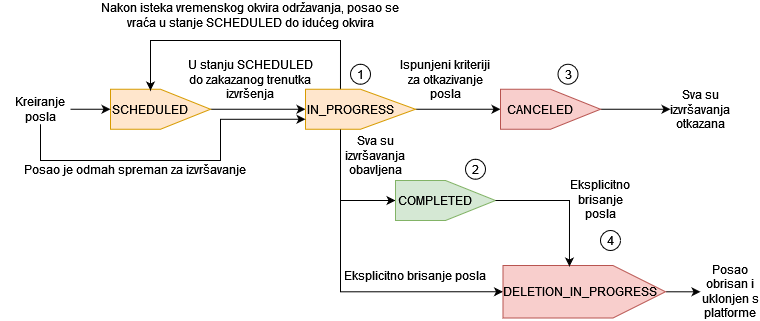
\includegraphics[scale=0.5]{imgs/job_states}
	\caption{Različita stanja tijekom izvršavanja posla \cite{aws_docs}}
	\label{fig:job_states}
\end{figure}

Postoje određena ograničenja na poslove i njihovo izvršavanje. Svi poslovi u stanju \textit{IN\_PROGRESS} smatraju se aktivnim poslovima za koje postoji limit. Ovo uključuje poslove koji ili uvode nova izvršavanja poslova ili poslove koji čekaju da uređaji dovrše postojeće izvršavanje. Ograničenje se odnosi na kontinuirane i jednokratne poslove. Poslovi u tijeku i poslovi koji poništavaju izvršenja prethodno stvorenih poslova istovremeni su i ubrajaju se u ograničenje istovremenosti poslova. Usluga može pokretati i otkazivati izvršenje poslova brzinom od tisuću uređaja u minuti. Svaki posao je istovremen i ubraja se u ograničenje istovremenosti poslova samo kratko vrijeme. Nakon što su izvršenja uvedena ili otkazana, posao više nije istovremen i ne ubraja se u ograničenje istovremenosti poslova. Moguće je iskoristiti istovremenost za kreiranje većeg broja poslova za vrijeme čekanja izvršenja postojećih poslova.

Isto tako, postoje različita stanja izvršenja samog posla. Izvršenje posla odnosi se na jednu instancu pokretanja posla na određenom ciljnom uređaju, te skup svih izvršenja poslova na svim uređajima određuje stanje samog posla. Tablica \ref{table:job_exec_states} prikazuje sva stanja u kojima se može naći izvršenje nekog posla. Isto tako, u tablici je navedeno koje stanje može okinuti uređaj, a koje usluga. Označeno je i koja su stanja prekidna, odnosno označavaju završetak izvođenja posla. Stupac \textit{retry} odnosi se na mogućnost ponovnog pokušaja izvršenja posla nakon navedenog stanja. 

\begin{table}[ht!]
	\centering
	\caption{Stanja izvršenja posla \cite{aws_docs}}
	\begin{tabular}{|c| c| c| c| c|}
		\hline
		\rowcolor{lightblue}  
		\textbf{Stanje} & \textbf{Pokrenuo uređaj?} & \textbf{Pokrenula usluga?} & \textbf{Prekidno?} & \textbf{\textit{Retry}?} \\ \hline
		\textit{QUEUED} & Ne & Da & Ne & - \\ \hline
		\textit{IN\_PROGRESS} & Da & Ne & Ne & - \\ \hline
		\textit{SUCCEEDED} & Da & Ne & Da & - \\ \hline
		\textit{FAILED} & Da & Ne & Da & Da \\ \hline
		\textit{TIMED\_OUT} & Ne & Da & Da & Da \\ \hline
		\textit{REJECTED} & Da & Ne & Da & Ne \\ \hline
		\textit{REMOVED} & Ne & Da & Da & Ne \\ \hline
		\textit{CANCELED} & Ne & Da & Da & Ne \\ \hline
	\end{tabular}
	\label{table:job_exec_states}
\end{table}

Kad usluga pošalje posao na ciljni uređaj, status izvršenja posla prelazi u \textit{QUEUED}. Posao stoji u stanju čekanja u redu sve dok uređaj ne primi izvršenje posla, pokrene ga i promijeni status u \textit{IN\_PROGRESS} koji zatim i pošalje na platformu. Isto tako, u slučaju da se posao otkaže ili se kriteriji otkazivanja posla ispune, status izvršenja posla prelazi u \textit{CANCELED}. Pri uspješnom izvršenju posla, uređaj šalje obavijest na platformu o uspješnosti, čime se status mijenja u \textit{SUCCEEDED}. Ako pak izvršenje posla bude neuspješno, prelazi u stanje \textit{FAILED} odakle ima priliku ponovnog izvršenja ako je tako naznačeno pri konfiguraciji samog posla. Stanje \textit{TIMED\_OUT} odnosi se na istek maksimalnog vremena izvođenja, i isto tako podržava mehanizam ponovnog izvršenja. Uređaj može promijeniti stanje izvršenja posla u \textit{REJECTED} ako primi nevaljan ili nekompatibilan zahtjev od platforme. Stanje \textit{REMOVED} postavlja se ako uređaj više nije podoban ili valjan za izvršenje traženog posla. 


\subsection{AWS IoT OTA}

\subsection{Ostale dostupne IoT usluge u sustavu AWS}

Uz ranije opisanu glavnu komponentu IoT Core koju nudi AWS za stvaranje IoT aplikacija, u samom ekosustavu nalazi se još mogućnosti za jednostavniju integraciju oblaka i fizičkih uređaja. U nastavku su ukratko opisane ostale usluge koje se mogu integrirati uz jezgrenu uslugu AWS IoT Core.

Važno je napomenuti kako nisu sve usluge dostupne u svim regijama unutar platforme AWS.

\subsubsection{IoT Analytics}

AWS IoT Analytics automatizira korake potrebne za analizu podataka prikupljenih od IoT uređajima. Filtrira, transformira i obogaćuje podatke prije nego ih pohrani u vremensku bazu podataka za daljnju analizu. Moguće je postaviti uslugu da prikuplja podatke s uređaja samo koji su potrebni, vrši matematičke operacije i dopunjava podatke raznim metapodacima, primjerice o lokaciji. Zatim se podaci mogu analizirati koristeći ugrađeni sustav za pretraživanje koji koristi SQL sintaksu ili pak vršiti kompleksniju analizu koristeći usluge umjetne inteligencije. Isto tako, ova usluga nudi vizualizaciju podataka integracijom s dodatnom uslugom Amazon QuickSight. 

\subsubsection{IoT Device Defender}

AWS IoT Device Defender potpuna je usluga koja pomaže pri osiguranju IoT uređaja. Kontinuirano revidira IoT konfiguracije radi provjere jesu li sve u skladu s najboljim sigurnosnim praksama. Također pruža kontinuirano monitoriranje sigurnosnih metrika s uređaja i usluge AWS IoT Core kako bi se detektirale anomalije u ponašanju pojedinih uređaja. 

Ova usluga također omogućuje slanje alarma na konzolu AWS IoT sustava i na uslugu za monitoriranje Amazon CloudWatch. Koriste se ugrađene mitigacijske akcije kako bi se izolirali nesigurni uređaji.

\subsubsection{IoT Events}

AWS IoT Events usluga služi za praćenje događaja u sustavu. Ova usluga prati ulazne podatke s više IoT uređaja i aplikacija radi prepoznavanja uzoraka i pokretanja prikladnih operacija na određene događaje. Moguće je pratiti ne samo fizičke uređaje, nego i druge AWS aplikacije integrirane u IoT sustav.

\subsubsection{IoT FleetWise}

AWS IoT FleetWise jest usluga koja se koristi za prikupljanje podataka od vozila i njihovu organizaciju u oblaku. Prikupljeni se podaci mogu koristiti za poboljšanje kvalitete, performansa i autonomije vozila. Također podržava više različitih protokola i podatkovnih formata. Ova usluga pomaže pri transformaciji poruka niske razine \engl{low-level} u oblik čitljiv čovjeku i standardizira podatke radi lakše analize u oblaku. Moguće je također definirati vrstu podataka i trenutak u kojem se ti podaci šalju u oblak.

Kada su podaci o vozilu u oblaku, mogu se koristiti u aplikacijama koje analiziraju zdravlje vozila. Ove informacije mogu pomoći pri identifikaciji potencijalnih problema u održavanju i pri unapređenju naprednih tehnologija poput autonomne i asistirane vožnje integracijom strojnog učenja.

\subsubsection{IoT Greengrass}

AWS IoT Greengrass jest usluga otvorenog koda \engl{open source} za računarstvo na rubu \engl{edge computing} i u oblaku koja pomaže pri izradi, objavi i upravljanju IoT aplikacija na uređajima. Može se koristiti za omogućavanje uređajima lokalno reagiranje na podatke koje generiraju, pokretanje modela strojnog učenja za predikciju, te filtriranje i agregaciju podataka s uređaja. Omogućava uređajima da prikupljaju i analiziraju podatke ne u oblaku, nego ili na samom uređaju ili drugom mjestu koje je bliže izvorištu tih podataka. Također može komunicirati na siguran način s uslugom AWS IoT Core i izvoziti podatke u oblak. Karakteristika računarstva u rubu, koje omogućava ova komponenta, jest približavanje računanja izvorišnim uređajima, čime se poboljšava vrijeme odziva i štedi propusnost \cite{what_is_edge}.

\subsubsection{IoT Roborunner}

AWS IoT RoboRunner nova je usluga koja pruža infrastrukturu za optimizaciju robota iz jedne točke gledišta. Uz pomoć ove usluge moguće je izgraditi aplikacije za jednostavniji međusobni rad robota. Namijenjena je za industrijske robote i automatizirane sustave za olakšano upravljanje opremom. Pruža centralne repozitorije podataka za pohranu te podržava različite podatkovne formate od raznih robota i autonomnih sustava.

\subsubsection{IoT TwinMaker}

AWS IoT TwinMaker usluga je za kreiranje operativnih digitalnih dvojnika fizičkih i digitalnih sustava. Stvara digitalne vizualizacije koristeći mjerenja i analize iz raznih senzora i kamera radi praćenja stvarnog stanja i uvjeta u kojima se objekt, zgrada ili kompleks nalazi. Podaci iz stvarnog svijeta se mogu koristiti za dijagnostiku i ispravljanje pogrešaka ili pak optimizaciju operacija. 

Digitalni dvojnik \engl{digital twin} digitalna je reprezentacija sustava i svih njegovih fizičkih i digitalnih komponenti. Dinamički se ažurira primitkom novih podataka kako bi simulirao stvarno stanje i ponašanje sustava. 


\subsubsection{IoT SiteWise}

AWS IoT SiteWise jest usluga koja skalabilno prikuplja, modelira, analizira i vizualizira podatke iz industrijske opreme. Usluga pruža kreiranje web aplikacija za operativne korisnike radi prikaza i analize industrijskih podataka u stvarnom vremenu. Moguće je dobiti uvide u podatke i operacije konfiguriranjem i praćenjem raznih metrika, primjerice efektivnost i efikasnost opreme. Ovu je uslugu moguće koristiti jedino uz ranije opisan IoT TwinMaker.

\eject
\chapter{Povezivanje razvojnog sustava i oblaka}

Oblak koju pruža platforma AWS i razvojni sustav ESP32-C3 dva su odvojena sustava koja moraju međusobno komunicirati i razmjenjivati podatke. Za ostvarenje njihove veze razvijena su dva programska rješenja:
\begin{enumerate}
	\item programska potpora za mikrokontroler, koja će omogućiti dinamičko povezivanje na Wi-Fi, spajanje na platformu AWS te slanje podataka u oblak,
	\item programska potpora za platformu AWS, koja će ostvariti umrežavanje uređaja u sustav, ažuriranje softvera na uređaju, pohranu primljenih podataka s uređaja te prikaz tih podataka u web aplikaciji. 
\end{enumerate} 

\section{Programska potpora za mikrokontroler}

Programska potpora za uređaj ESP32-C3 sastoji se od nekoliko komponenti:
\begin{itemize}
	\item dinamičko povezivanje na bežičnu mrežu,
	\item spajanje na platformu AWS,
	\item učitavanje novog softvera, 
	\item očitavanje senzorskih mjerenja, 
	\item slanje podataka u oblak protokolom MQTT.
\end{itemize}

Neke od navedenih komponenti izvršavaju se slijedno, dok se druge izvršavaju paralelno. Spajanje na Wi-Fi i povezivanje s platformom AWS ključni su koraci koji prethode bilo kakvom pokušaju slanja podataka u oblak. Isto tako, praćenje ažuriranja softvera i očitavanje mjerenja izvršavaju se paralelno u posebnim procesima budući da nisu sekvencijalni niti međusobno isključivi zadaci. U nastavku je pobliže opisan svaki navedeni segment programske potpore. 

\subsection{Dinamičko povezivanje mikrokontrolera na Wi-Fi}

Radni okvir ESP-IDF nudi dinamičko spajanje na Wi-Fi mrežu pomoću zasebne komponente. Ovaj se postupak naziva provizioniranje \engl{provisioning}. Ova komponenta pruža aplikacijska programska sučelja \engl{Application Programming Interface - API} koja kontroliraju pružanje usluge za primanje i konfiguriranje Wi-Fi vjerodajnica putem sigurnih komunikacijskih protokola. Sigurnosni protokoli definirani su u komponenti protokolne komunikacije \engl{protocomm} koja upravlja sigurnim sjednicama \engl{sessions} i pruža radni okvir za višestruki prijenos podataka. Također je moguće direktno koristiti sloj protokolne komunikacije radi implementacije specifične za aplikaciju \cite{unified_provisioning}.

Sloj protokolne komunikacije interno koristi mehanizam protokolnih međuspremnika \engl{protocol buffers - protobuf} za sigurno uspostavljanje sjednice. Protokolni međuspremnici namijenjeni su za serijalizaciju strukturiranih podataka neovisno o programskom jeziku i platformi. Koristan je pri izradi programa i sustava koji međusobno komuniciraju putem mreže zbog kompaktnosti i niske latencije \cite{what_is_protobuf}.

Sloj protokolne komunikacije pruža radni okvir za različite načine komunikacije:
\begin{enumerate}
	\item protokol BLE,
	\item Wi-Fi (SoftAP u kombinaciji s HTTP serverom).
\end{enumerate}

Pružajući korisnicima okvir za ostvarivanje usluge dinamičkog povezivanja u mrežu, neovisno o načinu komunikacije, ovakva vrsta podrške naziva se unificirano provizioniranje \engl{unified provisioning}. Ovakav način prijave uređaja na mrežu zahtijeva interakciju korisnika putem vanjskog uređaja za slanje vjerodajnica na mikrokontroler. Tvrtka \textit{Espressif} pruža jednostavna mobilna rješenja koja se mogu koristiti gotova ili pak uklopiti u vlastitu mobilnu aplikaciju. Na slici \ref{fig:unified_provisioning} prikazana je arhitektura usluge.

\begin{figure}[ht]
	\centering
	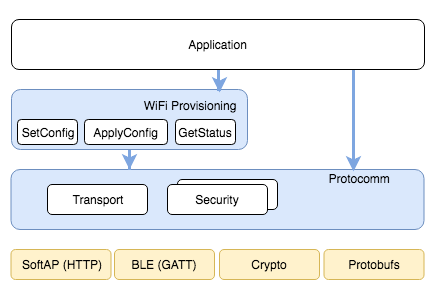
\includegraphics[scale=0.8]{imgs/unified_provisioning}
	\caption{Arhitektura unificiranog provizioniranja \cite{unified_provisioning}}
	\label{fig:unified_provisioning}
\end{figure}

Kao što je ranije opisano, arhitektura je bazirana na sloju protokolne komunikacije koji je odgovoran za prijenos podataka i sigurnost. Služi za jednostavne povratne pozive aplikaciji \engl{callbacks} i dobivanje Wi-Fi statusa. Sama aplikacija ima kontrolu nad implementacijom povratnih poziva. 

Aplikacija stvara instancu protokolne komunikacije koja se preslikava na određeni prijenosni protokol i sigurnosnu shemu. Svaki prijenos podataka u sloju protokolne komunikacije ima koncept krajnje točke \engl{endpoint} koji odgovara logičkom komunikacijskom kanalu za određenu vrstu informacija. Primjerice, sigurnosno rukovanje \engl{handshake} odvija se na različitoj krajnjoj točki u odnosu na točku za Wi-Fi konfiguraciju. Svaka se krajnja točka identificira nizom znakova i mijenja se ovisno o internom prikazu krajnje točke. U slučaju prijenosa pomoću Wi-Fi veze odnosno SoftAP funkcionalnosti, krajnja točka prikazuje se kao URI, dok u slučaju prijenosa podataka putem protokola BLE odgovara GATT karakteristici sa specifičnim identifikatorom. 

Oglašavanje i otkrivanje uređaja prepušteno je aplikaciji i ovisno o odabranom protokolu, vanjske aplikacije mogu odabrati odgovarajuću metodu za oglašavanje i otkrivanje. Za Wi-Fi prijenos obično se koristi ime mreže pristupne točke. Za prijenos putem protokola BLE može se koristiti ime samog uređaja. 

Kao što je opisano, podržano je korištenje protokola BLE kao i Wi-Fi usluge za prijenos vjerodajnica. Pri odabiru prijenosnog kanala za spajanje uređaja u mrežu, potrebno je razmotriti nekoliko točaka. Za početak, prijenos temeljen na protokolu BLE prednost održavanja netaknutog komunikacijskog kanala između uređaja i klijenta tijekom prijenosa podataka, što osigurava pouzdanu povratnu informaciju. S druge strane, prijenos putem Bluetootha troši oko 110 KB memorije tijekom rada, što je na uređajima niskih resursa velika potrošnja. Korisno je što se korištena memorija može vratiti na hrpu \engl{heap} po završetku umrežavanja uređaja ukoliko se BLE funkcionalnosti više ne koriste. Prijenos temeljen na Wi-Fi mreži, odnosno SoftAP funkcionalnosti, vrlo je interoperabilan i ne troši dodatnu memoriju. Međutim, mikrokontroler koristi isti radio za emitiranje pristupne točke i za spajanje na željenu mrežu. Budući da se te akcije mogu odvijati na različitim kanalima, postoji mogućnost da se ažuriranja statusa veze ne dostave na mobilni uređaj. Također, mobilni se uređaj mora odspojiti s izvorne Wi-Fi mreže radi privremenog spajanja na pristupnu točku mikrokontrolera. Uređaj će se spojiti na izvornu mrežu tak kada mikrokontroler ugasi pristupnu točku \cite{unified_provisioning}. 

Za razvoj predloženog rješenja korišteno je slanje vjerodajnica pomoću Wi-Fi mreže, odnosno privremene pristupne točke. Kao što je ranije opisano, protokol BLE troši značajnu količinu \textit{heap} memorije, a razvojni sustav ESP32-C3 nema dovoljno radne memorije koja bi pokrila prijavu u mrežu uz ostale radne procese. Mikrokontroler najprije stvori privremenu pristupnu točku na koju se mobilni uređaj spaja pomoću mobilne aplikacije. Zatim, nakon skeniranja dostupnih Wi-Fi mreža u blizini, u mobilnoj aplikaciji odabire se željena mreža i unese lozinka. Vjerodajnice se zatim pošalju putem Wi-Fi mreže, i mobilni uređaj može se odspojiti s privremene pristupne točke. Vjerodajnice se pohrane u memoriju tipa NVS \engl{non-volatile storage} koja ne zahtijeva konstantno napajanje kako bi se zadržala na uređaju. Ovime je omogućeno povezivanje uređaja u sustav čak i kada dođe do prekida napajanja \cite{what_is_nvs}. Memorija tipa NVS može se jedino programski obrisati, te bi u idealnom izvedbenom rješenju postojao vanjski gumb spojen na mikrokontroler koji bi pokretao brisanje te memorije i tako omogućio ponovno spajanje na željenu mrežu. Sljedeći programski isječak prikazuje inicijalizaciju memorije NVS, mrežnog sučelja te stvaranje pristupne točke.

\begin{lstlisting}[caption={Stvaranje pristupne točke}, language=c]
	/* Init NVS partition */
	esp_err_t ret = nvs_flash_init();
	/* Init TCP/IP */
	ESP_ERROR_CHECK(esp_netif_init());
	/* Init the event loop */
	ESP_ERROR_CHECK(esp_event_loop_create_default());
	wifi_event_group = xEventGroupCreate();
	/* Init Wi-Fi including netif with default config */
	esp_netif_create_default_wifi_sta();
	esp_netif_create_default_wifi_ap();
	wifi_prov_mgr_config_t config = {
		.scheme = wifi_prov_scheme_softap,
		.scheme_event_handler = WIFI_PROV_EVENT_HANDLER_NONE
	};
    /* Init provisioning manager with above config */
	ESP_ERROR_CHECK(wifi_prov_mgr_init(config));
	ESP_ERROR_CHECK(wifi_prov_mgr_start_provisioning(security, (const void *) sec_params, service_name, service_key));
	wifi_prov_print_qr(service_name, username, pop, PROV_TRANSPORT_SOFTAP, disp);
\end{lstlisting}

\subsubsection{LCD zaslon}

Za povezivanje mobilnog uređaja na privremenu pristupnu točku koju emitira razvojni sustav, potrebno je skenirati QR kod koji mikrokontroler generira. Budući da ESP32-C3 nema vlastito sučelje, na sustav je spojen zaslon OLED SSD1306 veličine 128×64 piksela. Uređaj sa zaslonom komunicira putem I2C sučelja, a za prikaz sadržaja na zaslonu korištena je biblioteka LVGL \engl{Light and Versatile Graphics Library}. To je grafička biblioteka otvorenog koda namijenjena izradi aplikacija s grafičkim korisničkim sučeljem \engl{Graphical User Interface - GUI} za ugradbene sustave. Pruža radni okvir s mnogim značajkama, temama i paletama boja. Isto tako, biblioteka troši vrlo malo resursa, što je čini pogodnom za uređaje poput razvojnog sustava ESP32-C3 \cite{lvgl}. Generiranje QR koda obavlja se pomoću biblioteke \textit{QR-Code-Generator} koja je prilagođena ESP32 uređajima. 

\begin{lstlisting}[caption={Generiranje QR koda iz pristupne točke}, language=c]
static void wifi_prov_print_qr(const char *name, const char *usrname, const char *pop, const char *transport, lv_disp_t *disp) {
	char payload[150] = {0};
    snprintf(payload, sizeof(payload), 	
    	"{\"ver\":\"%s\",\"name\":\"%s\",\"username\":\"%s\",\"pop\":\"%s\",\"transport\":\"%s\"}",
    	 PROV_QR_VERSION, name, usrname, pop, transport);
    esp_qrcode_config_t cfg = {
		.display_func = generate_qr_code_lcd, 
		.max_qrcode_version = 10, 
		.qrcode_ecc_level = ESP_QRCODE_ECC_LOW
	};
	esp_qrcode_generate(&cfg, payload);
}
\end{lstlisting}

Prethodna funkcija povezuje pristupnu točku s QR kodom. Podaci o samoj pristupnoj točki učitaju se u privremenu varijablu, čiji se sadržaj prosljeđuje biblioteci za generiranje QR koda. Dobiveni se podaci zatim prosljeđuju funkciji za prikaz koda na zaslonu. QR kod prikazuje se na zaslonu piksel po piksel, skalirajući veličinu QR koda na temelju širine i duljine samog zaslona. 

\begin{lstlisting}[caption={Funkcija za prikaz QR koda na zaslonu}, language=c]
void generate_qr_code_lcd(esp_qrcode_handle_t qrcode)
{
	ESP_LOGI(TAG, "%s", "Started generate_qr_code_lcd...");
	
	int size = qrcodegen_getSize(qrcode);
	
	// Calculate the scale factor
	int scale = (int)fmin(EXAMPLE_LCD_H_RES / size, EXAMPLE_LCD_V_RES / size);
	
	// Calculate horizontal shift
	int shift_x = (EXAMPLE_LCD_H_RES - size * scale)/2;
	
	// Calculate vertical shift
	int shift_y = (EXAMPLE_LCD_V_RES - size * scale)/2;
	
	if (lvgl_port_lock(0)) {
		lv_obj_t *screen = lv_scr_act();
		lv_obj_clean(screen); // Clear the screen to ensure it's dark
		
		// Create a canvas object
		lv_obj_t *canvas = lv_canvas_create(screen);
		static lv_color_t cbuf[LV_CANVAS_BUF_SIZE_TRUE_COLOR(EXAMPLE_LCD_H_RES, EXAMPLE_LCD_V_RES)];
		lv_canvas_set_buffer(canvas, cbuf, EXAMPLE_LCD_H_RES, EXAMPLE_LCD_V_RES, LV_IMG_CF_TRUE_COLOR);
		lv_canvas_fill_bg(canvas, lv_color_white(), LV_OPA_COVER);
		
		// Draw the QR code on the canvas
		for (uint8_t y = 0; y < size; y++) {
			for (uint8_t x = 0; x < size; x++) {
				if (qrcodegen_getModule(qrcode, x, y)) {
					for (int dy = 0; dy < scale; dy++) {
						for (int dx = 0; dx < scale; dx++) {
							lv_canvas_set_px(canvas, shift_x + x * scale + dx, shift_y + y * scale + dy, lv_color_black());
						}
					}
				}
			}
		}
		
		// Release the mutex
		lvgl_port_unlock();
	}
}
\end{lstlisting}

Na slikama \ref{fig:esp_softap_app1} i \ref{fig:esp_softap_app2} prikazana je mobilna aplikacija te trenutak nakon skeniranja QR koda. Mobilni uređaj zahtijeva spajanje na privremenu pristupnu točku, a iduća slika prikazuje dostupne Wi-Fi mreže u blizini mobilnog uređaja, ujedno i mikrokontrolera, na koje se razvojni sustav može spojiti. Odabirom jedne od mreža i unosom lozinke vjerodajnice se šalju na razvojni sustav.

\begin{figure}[ht]
	\begin{minipage}[t]{0.3\textwidth}
		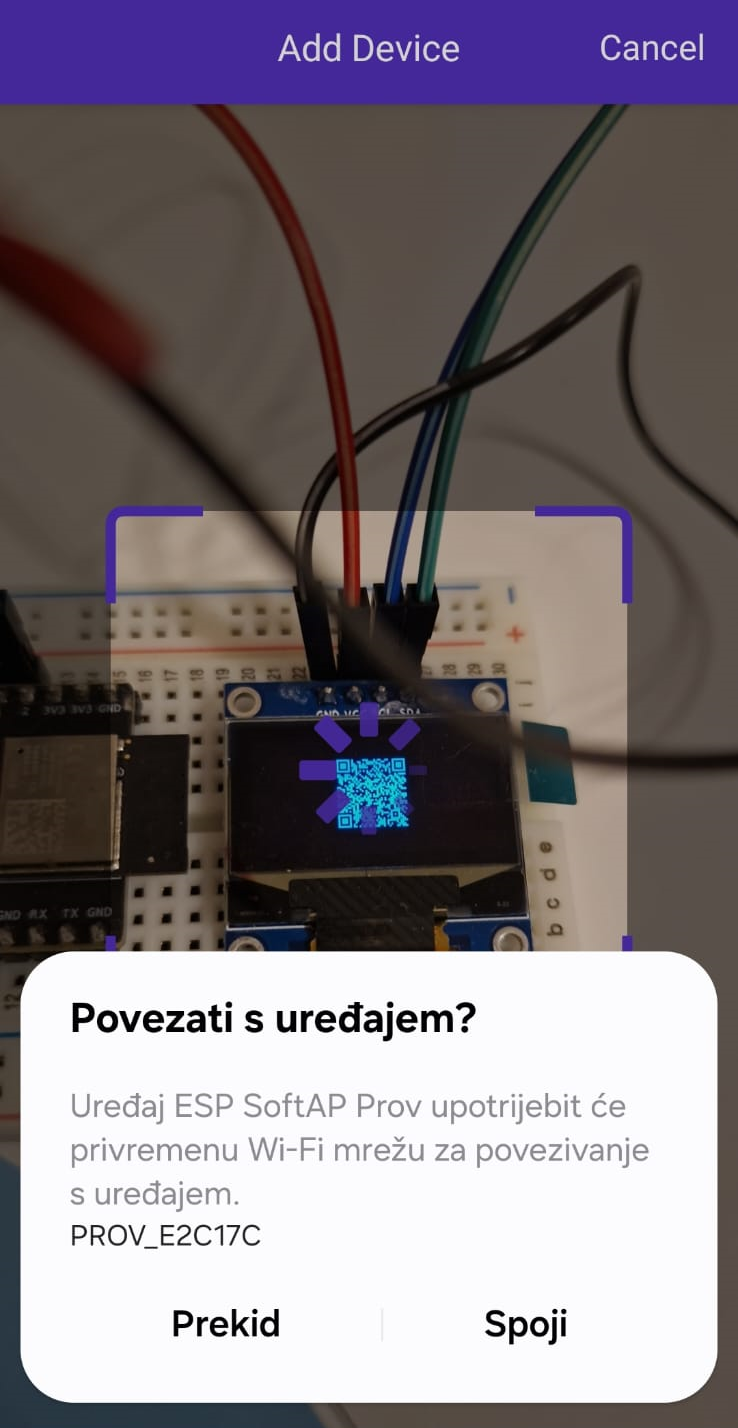
\includegraphics[width=\linewidth]{imgs/esp_softap_app1}
		\caption{Obavijest nakon skeniranja QR koda}
		\label{fig:esp_softap_app1}
	\end{minipage}
	\hspace*{\fill}
	\begin{minipage}[t]{0.3\textwidth}
		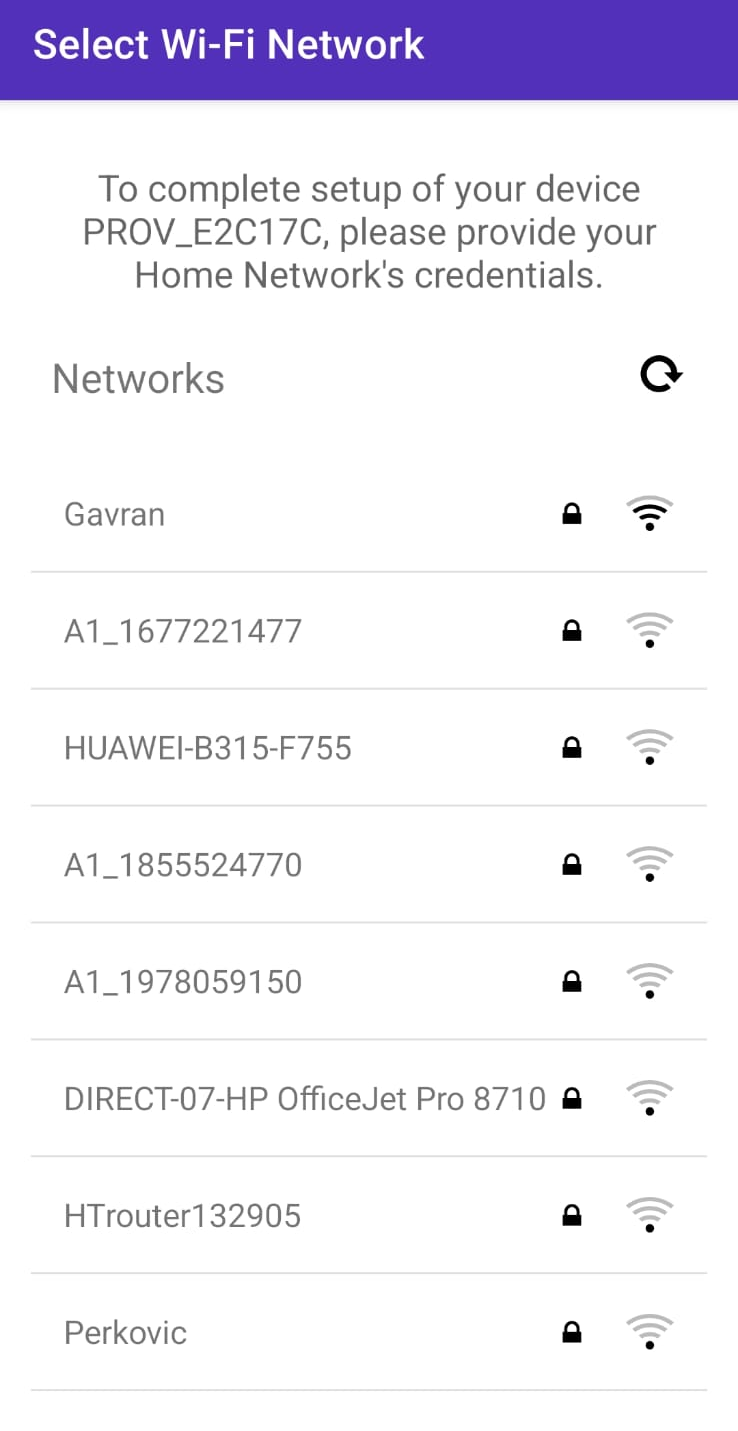
\includegraphics[width=\linewidth]{imgs/esp_softap_app2}
		\caption{Odabir dostupne Wi-Fi mreže u blizini}
		\label{fig:esp_softap_app2}
	\end{minipage}
\end{figure}

\subsection{Registracija u sustav AWS}

Nakon uspješnog povezivanja na Wi-Fi, sljedeći je korak registracija uređaja na platformu AWS. Korištena je biblioteka za AWS IoT Fleet Provisioning koja se održava u sklopu projekta otvorenog koda \textit{FreeRTOS} \cite{fleet_prov_sdk}. Biblioteka omogućuje mnoštvu odn. floti IoT uređaja registraciju i instalaciju jedinstvenih certifikata na platformu. Bibliotekom je moguće uređaje registrirati i pomoću autoriziranog korisnika, ali i certifikatima zahtjeva. Ova biblioteka ne ovisi o dodatnim bibliotekama osim standardne C biblioteke i stoga se može koristiti s bilo kojom bibliotekom za MQTT protokol.

Za potrebe ovog sustava odabrana je registracija pomoću certifikata zahtjeva. Na slici \ref{fig:fleet_provisioning_by_claim} prikazan je slijed događaja pri registraciji uređaja. Uređaj se najprije spaja na AWS certifikatom zahtjeva koji unaprijed postoji na mikrokontroleru te ostvaruje MQTT vezu. Zatim objavljuje praznu poruku na temu \textit{\$aws/certificates/create/json}, kojom zapravo podnosi zahtjev za kreiranjem vlastitog jedinstvenog certifikata. Usluga kreira traženi certifikat, pripadni ključ te generira značku vlasništva \engl{ownership token}, što sve skupa i objavljuje na temu \textit{\$aws/certificates/created/json/accepted}, na koju je uređaj pretplaćen. Razvojni sustav zatim sigurno pohranjuje dobivene vjerodajnice te objavljuje vlastite parametre i dobivenu značku na temu predloška za registraciju. Ako je kreirana, u sustavu AWS zatim se pokreće Lambda funkcija koja obavlja dodatne provjere nad dobivenim parametrima i tako provjerava valjanost zahtjeva. Primjerice, uređaj pri slanju parametara šalje i hardversku tajnu, koja se može zatim provjeriti u bazi podataka sustava AWS s pohranjenim takvim tajnama i provjeriti valjanost te tajne. Pri uspješnoj provjeri, Lambda funkcija vraća \lstinline|{"allowProvisioning" : True}|, čime daje konačno zeleno svjetlo za registraciju. Usluga posljedično kreira stvar i pripadnu politiku definiranu u predlošku te aktivira novostvoreni certifikat. Objavljuje novu konfiguraciju specifičnu za uređaj na temu za potvrdu uspješne registracije. Razvojni se sustav, nakon primjene nove konfiguracije, povezuje jedinstvenim privatnim ključem te certifikatom na AWS. Ova se nova MQTT veza dalje koristi za komunikaciju i razmjenu podataka.

\begin{figure}[ht]
	\centering
	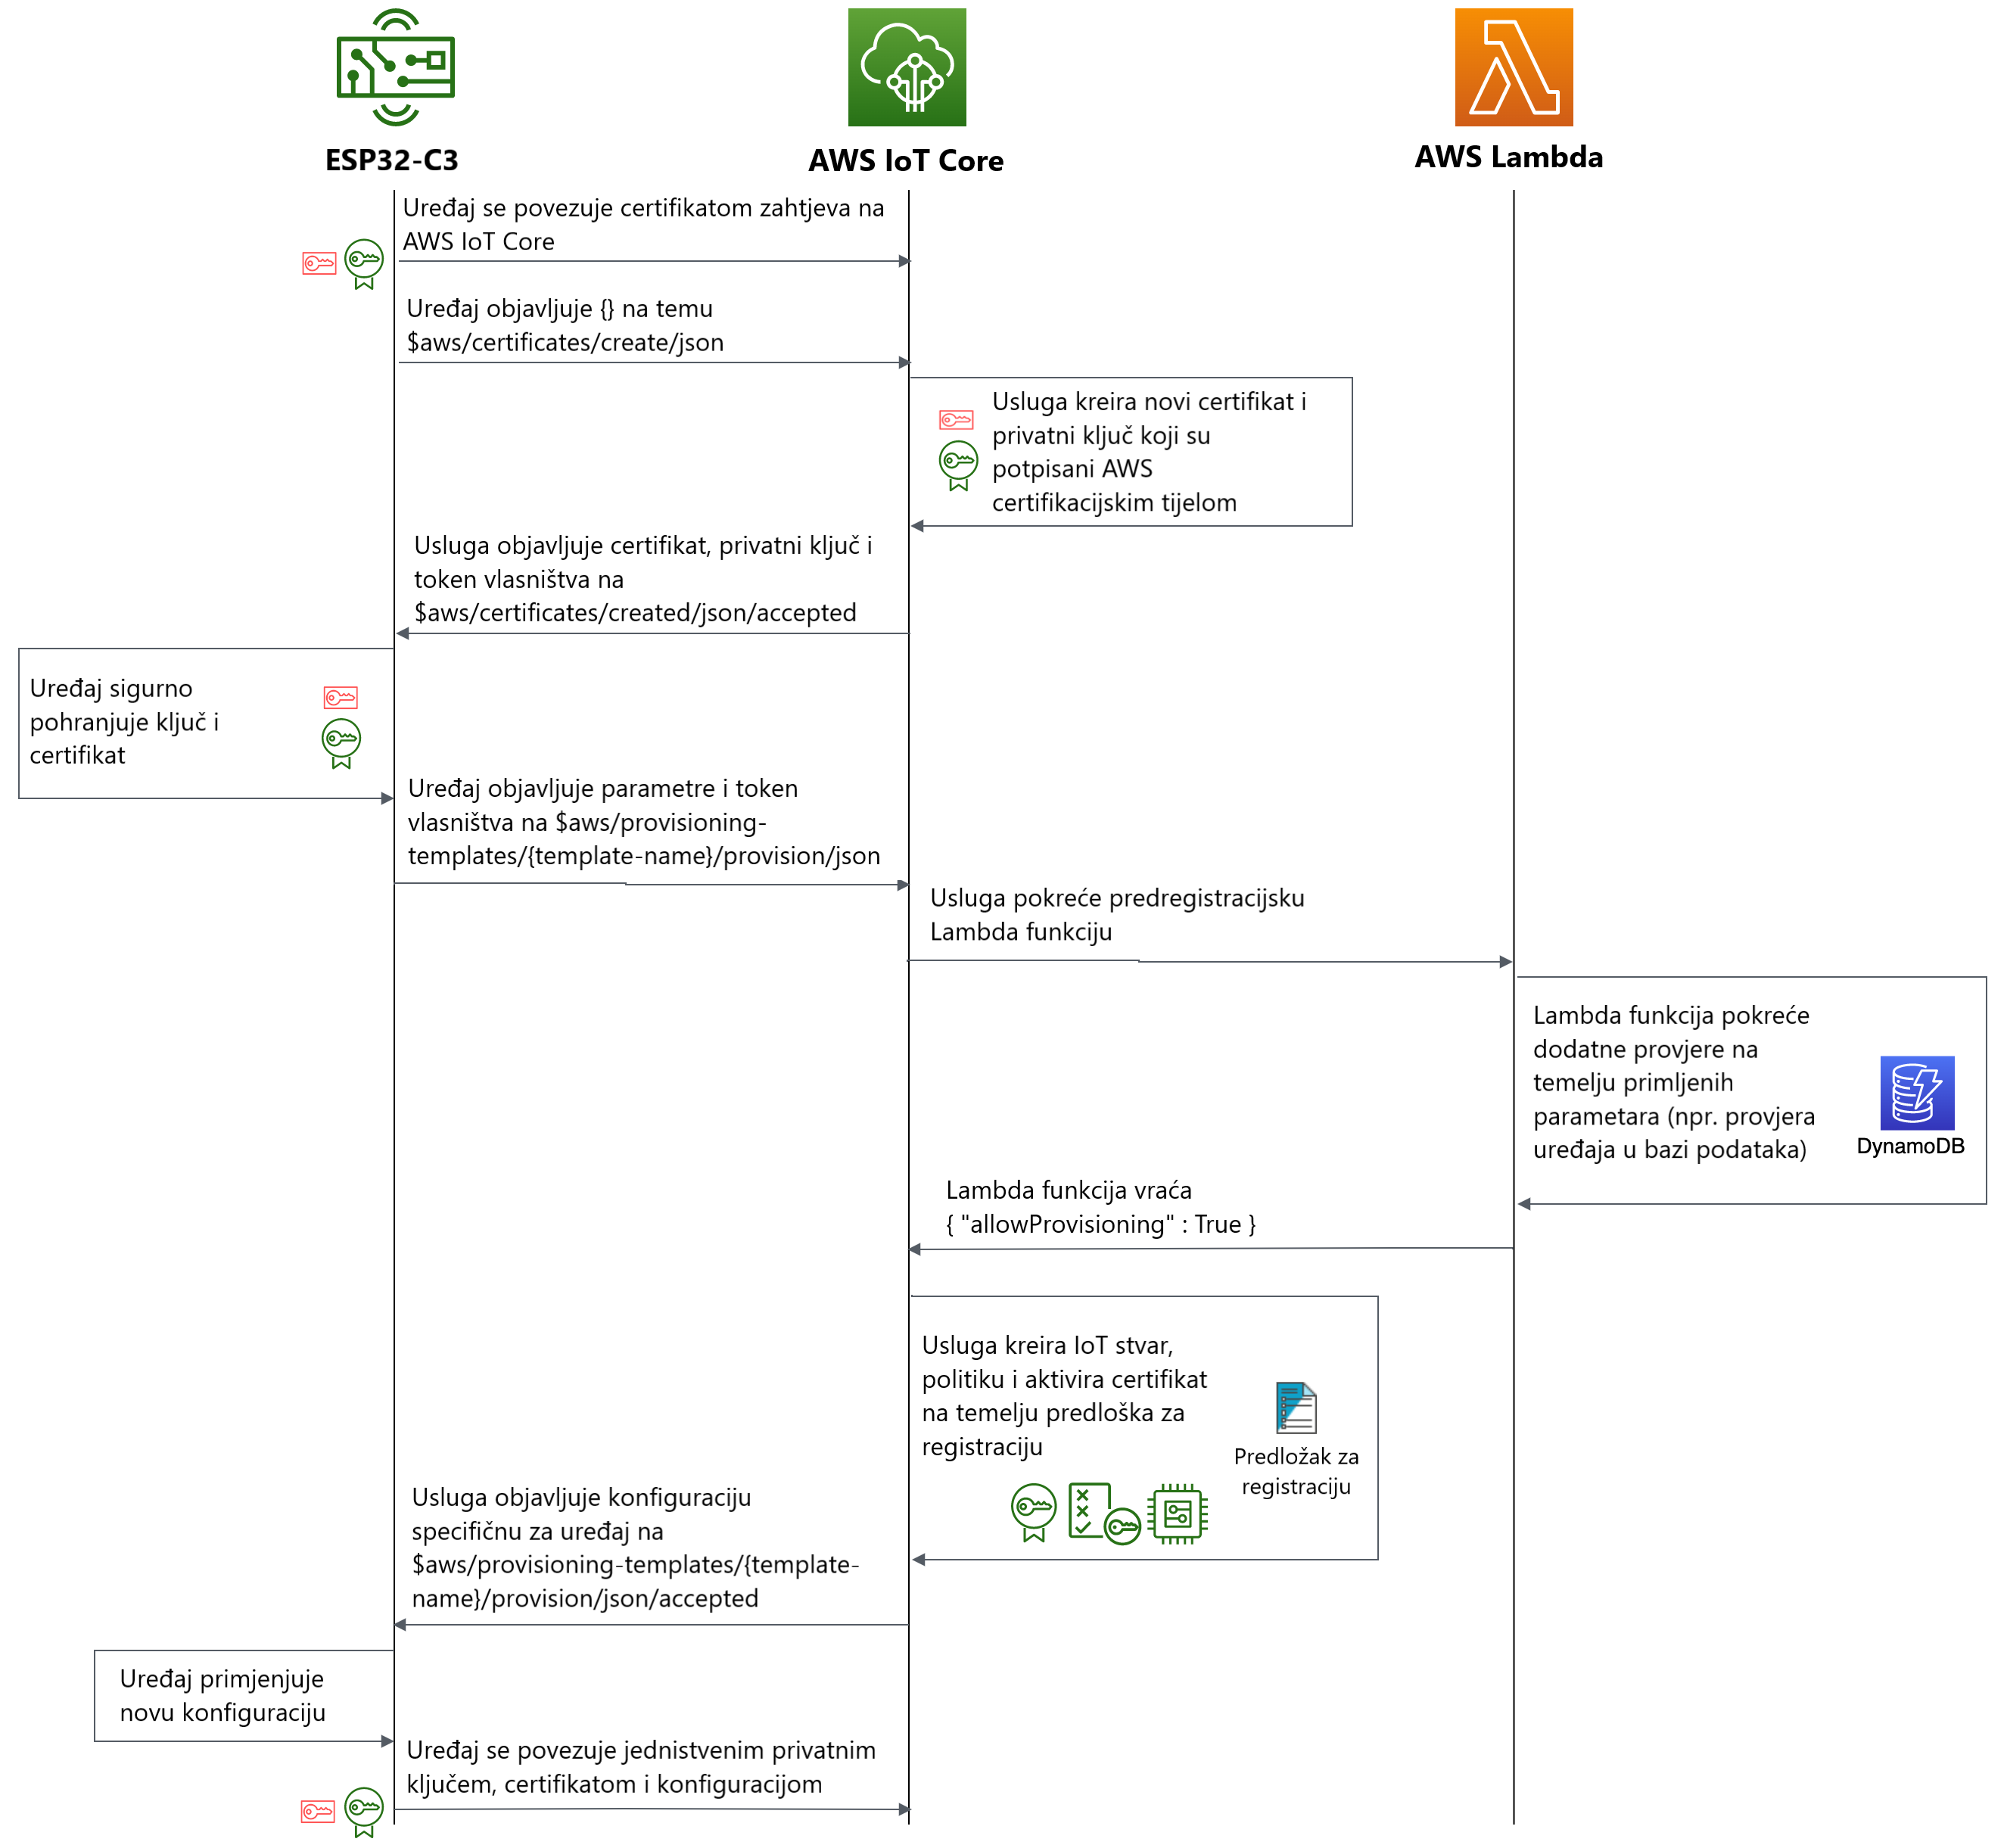
\includegraphics[scale=0.2]{imgs/fleet_provisioning_by_claim}
	\caption{Tok registracije uređaja certifikatom zahtjeva \cite{aws_docs}}
	\label{fig:fleet_provisioning_by_claim}
\end{figure}

Opisani tok ostvaren je uz pomoć ranije spomenute biblioteke, kao i knjižice \textit{coreMQTT} za komunikaciju putem protokola MQTT s API-jem platforme AWS. Za manipulaciju certifikatima i privatnim ključevima, korištena je biblioteka \textit{corePKCS11}. Ona koristi standard PKCS \#11 \engl{Public-key Certificate Standards}, što je široko korišten API za manipuliranje uobičajenim kriptografskim objektima. Funkcije koje navodi omogućuju aplikacijama korištenje, stvaranje, modificiranje i brisanje kriptografskih objekata, bez izlaganja tih objekata memoriji aplikacije. Primjerice, konkretna integracija s bibliotekom za registraciju uređaja koristi mali podskup PKCS \#11 API-ja za, između ostalog, pristup privatnom ključu potrebnom za stvaranje mrežne veze koja je autentificirana i zaštićena protokolom TLS bez da aplikacija ikada dođe u doticaj s ključem \cite{what_is_pkcs}. 

Sljedeći programski odsječak prikazuje uspostavu MQTT sjednice pomoću certifikata zahtjeva te podnošenje zahtjeva za novim certifikatom. U odsječku se također može primijetiti binarna serijalizacija podataka. Format CBOR \engl{Concise Binary Object Representation} Representation), za razliku od formata JSON, pretvara podatke u binarni oblik te ih tako šalje mrežom, što rezultira manjom latencijom i nosivošću \engl{payload} \cite{cbor}. Pri prijenosu velike količine podataka pri ograničenim resursima, poput u IoT sustava, ušteda na veličini poslanih podataka znatno utječe na efikasnost sustava. Isto tako, binaran je format prilagodljiv u odnosu na JSON, gdje mora postojati unaprijed definirana shema za primitak podataka.

\begin{lstlisting}[caption={Spajanje certifikatom zahtjeva i zahtjev za novim certifikatom}, language=c]
 LogInfo( ( "Establishing MQTT session with claim certificate..." ) );
 status = EstablishMqttSession( provisioningPublishCallback,
		*p11Session,
		pkcs11configLABEL_CLAIM_CERTIFICATE,
		pkcs11configLABEL_CLAIM_PRIVATE_KEY );
 status = subscribeToCsrResponseTopics();
 status = generateKeyAndCsr( *p11Session,
		pkcs11configLABEL_DEVICE_PRIVATE_KEY_FOR_TLS,
		pkcs11configLABEL_DEVICE_PUBLIC_KEY_FOR_TLS,
		csr,
		CSR_BUFFER_LENGTH,
		&csrLength );
/* Publish the CSR to CreateCertificatefromCsr API. */
 PublishToTopic( FP_CBOR_CREATE_CERT_PUBLISH_TOPIC,
		FP_CBOR_CREATE_CERT_PUBLISH_LENGTH,
		( char * ) payloadBuffer,
		payloadLength );
 status = waitForResponse();
\end{lstlisting}

\subsection{Očitavanje senzorskih mjerenja}

Razvijeni sustav, osim zaslona, sadrži dva senzora koja mjere stanja iz okoline: senzor za temperaturu i vlagu zraka te senzor za vlažnost tla. Mjerenja ovih senzora šalju se na platformu AWS i simuliraju stvarna poljoprivredna mjerenja. Mjerenje temperature i vlage zraka vrši se pomoću senzora DHT11, dok se vlažnost tla mjeri senzorom VMA303. 

\subsection{Slanje očitanih podataka protokolom MQTT}

\subsection{Sjena uređaja}

\subsection{Ažuriranje softvera}

\section{Programska potpora za oblak}

Programska potpora za platformu AWS nije kod u standardnom smislu, no kako bi se uređaj i platforma uopće mogli komunicirati međusobno, potrebno je omogućiti povezivanje i komunikaciju na samoj platformi. Sva se komunikacija odvija u istoj AWS regiji. Zbog dostupnosti većine IoT usluga i relativne geografske bliskosti, korištena je regija \textit{eu-north-1} odnosno Stockholm, Švedska. 

Isto tako, važno je istaknuti kako se sve opisane radnje u sustavu AWS mogu izvršavati pomoću naredbenog retka platforme AWS \engl{Command-line interface - CLI}, no radi jednostavnosti i preglednosti, korišteno je korisničko sučelje platforme.

Programska potpora sastoji se od sljedećih segmenata:
\begin{itemize}
	\item omogućavanje dinamičke registracije uređaja,
	\item slanje novog softvera na uređaj,
	\item pristup zadnjem stanju uređaja nakon gubitka veze,
	\item obrada podataka dobivenih protokolom MQTT,
	\item pohrana podataka.
\end{itemize}

\subsection{Dinamička registracija uređaja}

Kao što je ranije opisano, u razvijenom sustavu koriste se certifikati zahtjeva za prvotno spajanje na platformu AWS, stoga je potrebno kreirati odgovarajući predložak za registraciju. Predložak također mora imati dodijeljenu politiku koja autorizira certifikat zahtjeva i ta se politika dodjeljuje generiranim certifikatima zahtjeva. Odabiru se politike koje omogućavaju točno onoliko koliko je potrebno za spajanje u sustav, a to su dopuštenja za MQTT komunikaciju i spajanje na AWS. Također, potrebno je odabrati koji su certifikati valjani kao zahtjev. Poželjno je i dodijeliti Lambda funkciju kao predregistracijsku provjeru dodatne valjanosti zahtjeva i poslanih parametara. Za razvijeni sustav nije kreirana Lambda funkcija, što znači da je svaki zahtjev automatski odobren. Isto tako, moguće je automatski pri registraciji uređaja kreirati i pripadnu stvar \engl{thing}, što je korisno za kasniju organizaciju i pregled certifikata. Svaka stvar može imati modularan naziv, ovisno o parametrima koji se pošalju. Za ovaj sustav postavljen je prefiks \textit{ESP32Thing\_} koji označava da su uređaji vrste ESP32, a ostatak naziva stvari ovisi o serijskom broju samog uređaja. To osigurava da svaki uređaj kreira jedinstvenu stvar u AWS-u. Moguće je odabrati i vrstu stvari \engl{thing type} koja će se automatski pridijeliti stvari, te u ovom slučaju kreirana je nova vrsta stvari naziva ESP32-C3. Stvarima se može dodijeliti i grupa, no u ovom sustavu nije bilo potrebe za kreiranjem dodatne grupe stvari budući da se povezuje samo jedna vrsta uređaja u sustav. Naposlijetku, potrebno je odabrati koje će se politike dodijeliti novogeneriranom jedinstvenom certifikatu, čime će uređaj dobiti pristup uslugama sustava AWS. Odabrane politike u ovom sustavu imaju sva dopuštenja radi lakše demonstracije funkcionalnosti. U nastavku se može vidjeti isječak kreiranog predloška, odnosno parametri stvari koja se kreira korištenjem predloška. U odsječku se isto tako može vidjeti funkcija za kreiranje imena stvari koja koristi predefinirani prefiks i serijski broj uređaja. 

\begin{lstlisting}[caption={Odjeljak \textit{stvar} u predlošku za registraciju}, language=json]
 "thing": {
	"Type": "AWS::IoT::Thing",
	"OverrideSettings": {
		"AttributePayload": "MERGE",
		"ThingGroups": "DO_NOTHING",
		"ThingTypeName": "REPLACE"
	},
	"Properties": {
		"AttributePayload": {},
		"ThingGroups": [],
		"ThingName": {
			"Fn::Join": [
			"",
			[ "ESP32Thing_", { "Ref": "SerialNumber" } ]
			]
		},
		"ThingTypeName": "ESP32-C3"
	}
 }
\end{lstlisting}

Na slici \ref{fig:policies} nalazi se popis politika koje su dodijeljene uređaju registriranom u sustav. Omogućene su sve politike, odnosno dodijeljene su sve dozvole koje uređaj može imati. Politika \textit{DevicePolicy} odnosi se na komunikaciju MQTT protokolom, \textit{DeviceShadowPolicy} na akcije vezane uz sjenu uređaja, \textit{JobPolicy} na izvršavanje i dohvat poslova te \textit{CertificatePolicy} dozvoljava povezivanje certifikatom. 

\begin{figure}[ht]
	\centering
	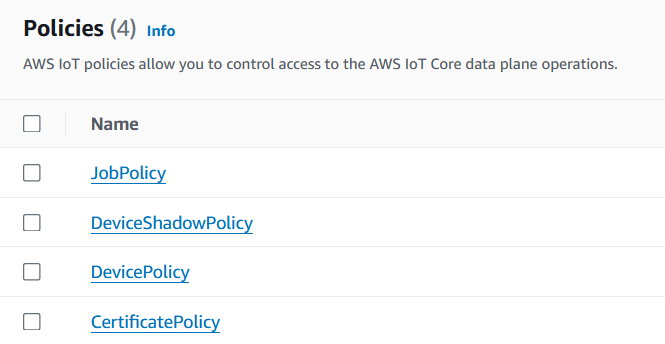
\includegraphics[scale=0.8]{imgs/policies}
	\caption{Popis politika dodijeljenih registriranom uređaju}
	\label{fig:policies}
\end{figure}

\chapter{Web aplikacija}

Svi podaci koji su pohranjeni u bazi podataka trebaju biti korisnicima na raspolaganju jednostavno i intuitivno. U tu je svrhu kreirana aplikacija radi prikaza i vizualizacije podataka korisnicima u stvarnom vremenu. Web aplikacija treba biti javno dostupna na internetu kako bi korisnici razvijenog sustava mogli pregledavati podatke poslane s uređaja. Za objavu web aplikacije na internet \engl{deployment} kreirani su vlastiti resursi na kojima se izvršava aplikacija. Za infrastrukturu aplikacije korišteni su resursi platforme AWS koji pružaju iznajmljivanje virtualnih računala te se na njima mogu pokrenuti vlastite računalne aplikacije. Za web aplikaciju koja će korisnicima pružati uvid u podatke odabrana je Grafana koja nudi brojne funkcionalnosti za vizualizaciju podataka. Nadalje, kreiran je i alarmni sustav koji obavještava o promjenama stanje koja dolaze od uređaja. 

\section{Infrastruktura aplikacije}

Temelj cijele infrastrukture aplikacije jest usluga Amazon EC2 \engl{Elastic Compute Cloud}. Ova usluga pruža skalabilni računalni kapacitet na zahtjev u oblaku platforme AWS. Ova usluga omogućava pokretanje neograničenog broja virtualnih poslužitelja, ovisno o zahtjevima aplikacije i razvijanog sustava, konfiguriranje sigurnosti i umrežavanja te upravljanje pohranom. Usluga EC2 nudi razne prednosti \cite{aws_docs}:
\begin{itemize}
	\item fleksibilno skaliranje: omogućava brzo povećanje ili smanje kapaciteta u kombinaciji s uslugom EC2 Auto Scaling za automatsko skaliranje radi prilagodbe troškova,
	\item potpuna kontrola nad instancom: pruža pristup instanci kao i bilo kojem stroju, moguće pokretanje i zaustavljanje spajanjem na udaljeno računalo, ali i API pozivom,
	\item fleksibilne usluge objave u oblaku: nudi izbor između više vrsta instanci, operacijskih sustava i softverskih paketa te nudi konfiguraciju memorije, procesora i pohrane,
	\item integracija s drugim uslugama: jednostavno se integrira s ostalim uslugama us sklopu platforme AWS,
	\item pouzdanost: nudi vrlo pouzdano okruženje u kojem se zamjenske instance mogu brzo pokrenuti, te je obaveza ugovora o razini usluge Amazon EC2 \engl{Service Level Agreement - SLA} dostupnost od 99,99\% za svaku regiju,
	\item sigurnost: arhitektura nudi različite sigurnosne značajke i postavljanje virtualnih privatnih mreža za ograničen pristup resursima.
\end{itemize}

EC2 instance virtualni su poslužitelji koji rade na infrastrukturi računalstva u oblaku tvrtke Amazon. Jedan fizički AWS poslužitelj uslužuje više EC2 virtualnih poslužitelja koje pokreće hipervizor na računalu domaćinu. Ova usluga pružanja virtualne infrastrukture dio je skupa IaaS usluga koje AWS nudi. EC2 virtualni poslužitelji kopije su izvornog predloška na kojem se temelje. AMI \engl{Amazon Machine Image} temeljna je komponenta koja omogućava pokretanje virtualnih poslužitelja u AWS infrastrukturi. Predstavlja virtualni stroj koji sadrži sve potrebne informacije za pokretanje instance, uključujući operacijski sustav, aplikacije te konfiguracijske podatke. To je prilagodljivi predložak za EC2 instance. Iz jednog AMI predloška, odnosno slike stroja, moguće je kreirati više istih EC2 instanci, što olakšava njihovo stvaranje i objavu na internet. Ovo je korisno za horizontalno skaliranje aplikacija. Slika \ref{fig:ami} prikazuje način na koji funkcionira AMI predložak - kreira instance bilo koje vrste te ih pokrene na domaćinskim računalima \cite{ec2}.

\begin{figure}[ht]
	\centering
	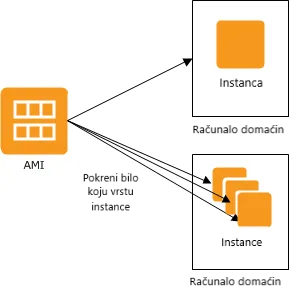
\includegraphics[scale=0.6]{imgs/ami}
	\caption{AMI predložak i distribucija slika stroja na instance \cite{ec2}}
	\label{fig:ami}
\end{figure}

AMI predlošci podržavaju dva tipa virtualizacije: hardversku virtualizaciju i paravirtualizaciju. Predložak s hardverskom virtualizacijom pruža mogućnost pokretanja operacijskog sustava izravno na vrhu virtualnog stroja bez ikakvih izmjena, kao da se pokreće na samom hardveru \engl{bare-metal hardware}. Domaćinski sustav usluge EC2 emulira dio ili sav temeljni hardver koji je predstavljen gostu odnosno AMI slici. Moguće je isto tako koristiti hardverska proširenja koji pružaju brzi pristup domaćinskom hardveru. Paravirtualizacija koristi poseban pokretački program koji lančano učitava jezgru u AMI sliku. Paravirtualni gosti mogu se pokretati na domaćinskom hardveru koji nema eksplicitnu podršku za virtualizaciju. Ovaj tip ne simulira hardver, nego pravi hiperpozive \engl{hypercalls} za izvršavanje osjetljivih CPU naredbi. Preporuča se odabir hardverske virtualizacije, iako generalno paravirtualizacija pruža bolje performanse, zbog poboljšanja hardverske virtualizacije i novih upravljačkih programa koji izjednačava rad obje vrste virtualizacije. 

Pri kreiranju instance potrebno je definirati i njezinu vrstu. Vrsta koja se navede određuje hardver dostupan instanci. Svaka vrsta nudi različitu ravnotežu računalnih, memorijskih i mrežnih resursa. Vrste su grupirane u skupine na temelju potreba ciljnih aplikacija. AWS pruža sljedeće vrste instanci:
\begin{itemize}
	\item opće namjene \engl{general purpose}, 
	\item optimiziranog računanja \engl{compute optimized},
	\item optimizirane memorije \engl{memeory optimized},
	\item optimizirane pohrane \engl{storage optimized}, 
	\item ubrzanog računanja \engl{accelerated computing},
	\item računanja visokih performansi \engl{high-performance computing}.
\end{itemize}

Vrstu instance potrebno je odabrati na temelju zahtjeva same aplikacije. Isto tako, pri kreiranju instance, uvijek je potrebno voditi računa o odabiru regije - optimalno je odabrati regiju kojoj je klijentski promet najbliži.

Za potrebe razvijenog sustava, kreirana je EC2 instanca opće namjene s najmanjim resursima budući da je klijentski promet jako malen, odnosno vrlo malo korisnika pristupa aplikaciji. Također, pridružena joj je instanca spremnika za pohranu veličine 8 GB. Operacijski sustav na kreiranoj instanci aplikacije jest Linux radi lakšeg spajanja na instancu i pokretanja web aplikacije putem komandne linije. Pri stvaranju instance kreirana je nova sigurnosna grupa koja omogućava spajanje na virtualno računalo putem SSH klijenta.

Instanci je automatski dodijeljena virtualna privatna mreža \engl{Virtual Private Cloud - VPC} koja predstavlja izolirani virtualni mrežni prostor unutar AWS infrastrukture. Omogućava potpunu kontrolu nad mrežnim okruženjem, uključujući izbor vlastitog IP adresnog prostora, konfiguraciju podmreža, postavljanje usmjeravanja i pristupnih kontrola mreže. Svaka je virtualna privatna mreža podijeljena na manje dijelove mreže zvane podmreže. One mogu biti privatne ili javne te se automatski za svaku mrežu kreiraju tri podmreže. Svaka je kreirana podmreža prema zadanim postavkama privatna, te je za pristup instanci odnosno aplikaciji koja se nalazi za njom potreban javni pristup. Iako omogućavanje javnog pristupa znači da svatko može pristupiti IP adresi instance s interneta, unošenje IP adrese pri svakom pristupu aplikaciji nije prilagođeno korisniku, što narušava korisničko iskustvo korištenja aplikacije. Stoga je potrebno uvesti komponentu za balansiranje opterećenja \engl{load balancer}. Balanseri preusmjeravaju korisničke zahtjeve na manje opterećene instance i tako ravnomjerno raspoređuju ulazni promet. Budući da je u razvijenom sustavu korištena samo jedna instanca na kojoj se pokreće aplikacija, ovdje je primarna svrha balansera pružiti DNS naziv koji će biti javno dostupan korisnicima, i tako poboljšati iskustvo korištenja aplikacije. 

Aplikacijskoj instanci potrebno je dodijeliti pravila za ulazne zahtjeve, odnosno omogućiti TCP komunikaciju s podmreže u kojoj se nalazi balanser. Tim se pravilom omogućuje prolaz zahtjeva s balansera prema aplikacijskoj instanci. Isto tako, iz sigurnosnih razloga poželjno je koristiti protokol HTTPS za pristup balanseru. Za korištenje protokola HTTPS potrebno je učitati certifikat, no budući da domena na kojoj se nalazi balanser nije službeno registrirana, ne posjeduje niti službeno potpisani certifikat. Stoga je lokalno kreiran samopotpisani certifikat pomoću biblioteke \textit{OpenSSL} i zatim učitan u oblak. Slika \ref{fig:load_balancer} prikazuje mrežnu povezanost balansera i instance na kojoj se nalazi aplikacija. Balanser sluša promet na vratima 443, što su vrata za protokol HTTPS. Dolazni zahtjevi prosljeđuju se skupini ciljnih instanci, ovdje pod nazivom \textit{GrafanaTargetGroup}, u kojoj se mogu nalaziti sve buduće stvorene instance na kojima se pokreće aplikacija. Nadalje, promet se prosljeđuje ciljnoj instanci koja je dostupna na vratima 3000. Na tim je istim vratima pokrenuta aplikacija. 

\begin{figure}[ht]
	\centering
	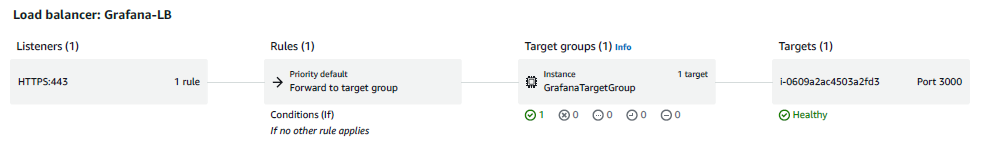
\includegraphics[scale=0.7]{imgs/load_balancer}
	\caption{Mrežna povezanost balansera i aplikacijske instance}
	\label{fig:load_balancer}
\end{figure}

Kako bi se maksimalno izoliralo izvođenje aplikacije i tako ostavilo prostora za izvršavanje drugih procesa na virtualnom računalu, na instanci EC2 aplikacija je pokrenuta pomoću alata Docker radi kontejnerizacije aplikacije. Sljedeći programski isječak prikazuje naredbu za preuzimanje i pokretanje Docker slike za Grafanu. Isto tako, potrebno je izložiti vrata na kojoj se pokreće aplikacija kako bi joj se moglo pristupiti. Grafana nudi dvije verzije - otvorenog koda i \textit{enterprise}, koja nudi više značajki. Za potrebe razvijenog sustava korištena je slika verzije otvorenog koda. Potrebno je također i postaviti varijable okoline za povezivanje s SMTP poslužiteljem \engl{Simple Mail Transfer Protocol}, koji će kasnije služiti za slanje e-pošte obavijesti. Korišten je poslužitelj koji dolazi uz uslugu Gmail tvrtke \textit{Google}, te je potrebno navesti aplikacijsku lozinku koja se može kreirati u Gmail računu.

\begin{lstlisting}[caption={Pokretanje Docker slike za Grafanu}, language=bash]
sudo docker run -d -p 3000:3000 --name grafana 
	-e "GF_SMTP_ENABLED=true" \
	-e "GF_SMTP_HOST=smtp.gmail.com:587" \
	-e "GF_SMTP_USER=gmail.address@gmail.com" \
	-e "GF_SMTP_PASSWORD=GeneratedPassord123" \
	grafana/grafana-oss
\end{lstlisting}

\section{Grafana}

Grafana je platforma otvorenog koda za vizualizaciju i analizu podataka koja omogućava korisnicima stvaranje interaktivnih i prilagodljivih nadzornih ploča \engl{dashboards}. Cilj platforme jest olakšati analize vremenskih nizova podataka te integrira podatke iz različitih izvora podataka \engl{data source}, što mogu biti različite baze ili sustavi. Nudi jednostavnu vizualizaciju pomoću različitih grafičkih elemenata, uključujući linijske, stupčaste i tortne grafove. Široko je korištena zbog svoje sposobnosti da prezentira podatke na intuitivan način, omogućujući korisnicima donošenje informiranih odluka na temelju stvarnim podataka u stvarnom vremenu. Također, Grafana nudi alarmni sustav koji se koristi za izvještavanje korisnika o promjenama u podacima \cite{grafana}. 

Grafana se najčešće koristi za nadzor infrastrukture, performansi aplikacija i poslovnih metrika. Često je korištena za praćenje stanja poslužitelja, mrežnog prometa i performansi aplikacija. Također se koristi u poslovnoj analitici za praćenje poslovnih metrika. Isto tako, Grafana je korisna za IoT sustave upravo zbog sposobnosti vizualizacije velike količine podataka u stvarnom vremenu. Količine podataka koje IoT uređaji generiraju moraju se analizirati kako bi se dobili uvidi u očitana mjerenja, zdravlje sustava, kao i same performanse uređaja. Upravo zbog jednostavnog povezivanja s više različitih izvora podataka, njome se ostvaruje središnje mjesto za praćenje i analizu podataka iz cijele IoT mreže. Koristeći interaktivne nadzorne ploče, moguće je pratiti očitanja sa senzora u stvarnom vremenu i kreirati mnoge vizualizacije ovisno o potrebama sustava. Također podržava složene upite i transformacije podataka, što omogućuje njihovu dubinsku analizu. Korištenjem grafičkih elemenata i filtriranja podataka, mogu se lako identificirati trendovi, obrasci i anomalije u podacima \cite{grafana_iot}.

Kako bi web aplikacija mogla prikazivati podatke iz baze InfluxDB, na Grafani je potrebno stvoriti izvor podataka koji će služiti kao spojnica aplikacije i baze. Kako bi Grafana koristila InfluxDB kao izvor, koristi se dodatak \engl{plugin} koji služi kao poveznica između dva sustava. Osim što omogućuje njihovo povezivanje na razini dohvaćanja podataka, istovremeno mapira vremenske okvire odabrane u Grafani u stvarne vremenske točke koje baza može parsirati. Budući da se u bazi nalaze dvije kante, \textit{esp32data} i \textit{esp32state}, za svaku je od njih potrebno napraviti poseban izvor podataka. Kako bi se Grafana uspješno spojila na bazu, potrebno je korisničko ime i lozinka, kao i token koji će omogućavati čitanje iz baze. U bazi InfluxDB kreiran je novi korisnik \textit{grafana} koji služi samo za potrebe web aplikacije i generirana su dva tokena, svaki za jednu kantu. Tokeni omogućavaju isključivo čitanje iz kante. Važno je također napomenuti kako se novi korisnici ne mogu kreirati putem sučelja baze InfluxDB, nego je potrebno lokalno preuzeti alat za upravljanje bazom te se udaljeno putem komandne linije spojiti na bazu InfluxDB i tako kreirati korisnika.

Za kreiranje upita prema bazi koristi se jezik Flux. To je skriptni jezik za podatke \engl{functional data scripting language} namijenjen postavljanju upita i analizi podataka vremenskih serija. Upiti mogu sadržavati agregacije i transformacije. Iako jezik dolazi sa predefiniranim skupom funkcija za rad nad vremenskim serijama, moguće je definirati i vlastite prilagođene funkcije. Većina upita u jeziku Flux prate jednaki slijed koji se lančano izvodi:
\begin{enumerate}
	\item definiranje izvora,
	\item filtriranje,
	\item oblikovanje,
	\item obrada. 
\end{enumerate}

Prvi korak je odabir izvora podataka, što se odnosi na izbor kante. Podaci su vraćeni u tabličnom obliku. Funkcije filtriranja iteriraju po svim redovima dobivene tablice i provjeravaju zadovoljavaju li unosi tražene kriterije. Primarne funkcije za filtriranje su \lstinline|range()| i \lstinline|filter()|. Prva funkcija filtrira podatke na temelju vremenskog okvira, dok \lstinline|filter()| filtrira vrijednosti na temelju sadržaja redaka. Koristi se predikatna funkcija definirana unutar izraza za evaluaciju retka. Svaki se redak predikatnoj funkciji prosljeđuje kao zapis koji sadrži parove ključ-vrijednost za svaki stupac u retku. Oblikovanje podataka odnosi se na grupiranje ili modifikaciju same strukture podataka prije slanja na daljnju obradu. Funkcija \lstinline|group()| grupira podatke na temelju danog ključa, \lstinline|window()| stvara skupine na temelju danih vremenskih okvira, dok \lstinline|keep()| i \lstinline|drop()| zadržavaju odnosno uklanjaju pojedine stupce. Funkcija \lstinline|pivot()| vrijednosti stupca pretvara u redak. Obrada podataka odnosi se nad sve ostale operacije manipulacije podacima: agregiranje, mapiranje, prepisivanje te odabir pojedinih točaka u vremenu \cite{influxdb}. 

Za potrebe razvijenog sustava, kreirana je nadzorna ploča koja prikazuje mjerenja pojedinih senzora: temperatura, vlažnost zraka i vlaga tla.  Svaka je vizualizacija predstavljena jednim panelom kojem je dodijeljen naziv i opis. Paneli mogu biti različite vrste grafova vremenskih serija, no mogu biti i tekst ili jedna vrijednost. Svaki je panel moguće stilizirati bojama, veličinom i debljinom linija. Također, filtriranjem i transformacijama vrijednosti mogu se dobiti nove varijable za prikazati na panelu. Ovisno o vrijednostima varijabli koje se nalaze na panelu, moguće je mijenjati izgled i boju samih grafova. Paneli se mogu grupirati u redove, ovisno o njihovom zajedničkom značaju. Također, važna značajka jest definiranje varijabli na razini nadzorne ploče. Moguće je korištenjem upita ili pak vlastitim proizvoljnim unosom definirati varijable koje se zatim mogu koristiti u svim panelima. Tako će korisnik, odabirom vrijednosti varijable, vidjeti i željena mjerenja odnosno grafove samo za one vrijednosti varijabli koje ga zanimaju.

Unutar nadzorne ploče kreirana je varijabla \textit{device\_id}, koja pruža odabir između postojećih serijskih brojeva odnosno identifikatora uređaja na temelju podataka u bazi. Tako se jednostavno može pregledati statistika samo za željeni uređaj na pregled, budući da je svaki panel povezan s definiranom varijablom. Isto tako, varijabla omogućava odabir i svih dostupnih vrijednosti, čime je omogućen pregled za sve uređaje odjednom. Naravno, podaci su na panelima i dalje grupirani po serijskom identifikatoru uređaja. U nastavku se nalazi upit koji je korišten za definiranje varijable \textit{device\_id}. Bojama su prikladno označene različite vrste funkcija upita. 

\begin{lstlisting}[caption={Upit za dohvat identifikatora uređaja}, language=flux]
from(bucket: "esp32data")
|> range(start: v.timeRangeStart, stop: v.timeRangeStop)
|> filter(fn: (r) => r._measurement == "esp32")
|> group(columns: ["device_id"])
|> map(fn: (r) => ({ device_id: r.device_id }))
\end{lstlisting}

\begin{figure}[ht]
	\centering
	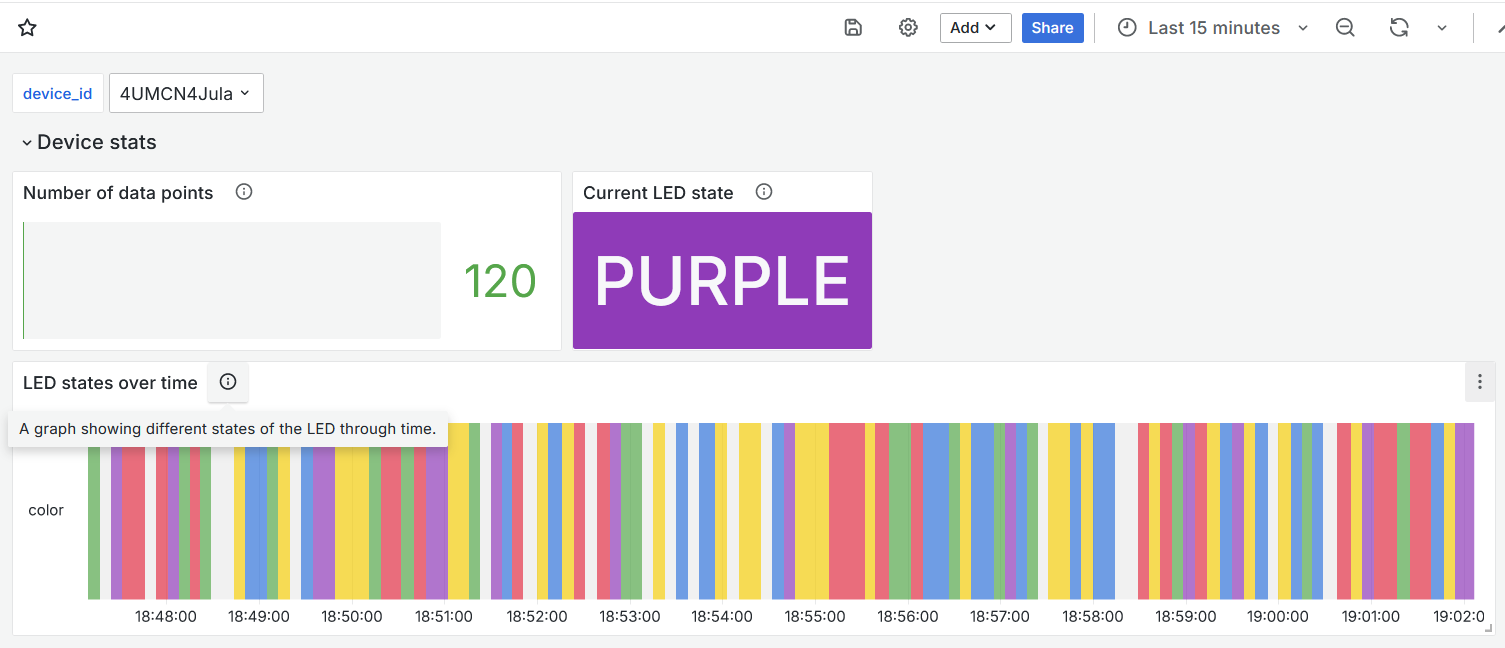
\includegraphics[scale=0.4]{imgs/grafana_device_stats}
	\caption{Prikaz stanja uređaja na Grafani u posljednjih petnaest minuta}
	\label{fig:grafana_device_stats}
\end{figure}

Slika \ref{fig:grafana_device_stats} prikazuje red nadzorne ploče koji sadrži panele stanja uređaja tijekom posljednjih petnaest minuta. Odabran je jedan identifikator uređaja, stoga se prikazuju podaci samo za taj jedan uređaj. Prvi panel prikazuje koliko se ukupno vremenskih točaka nalazi u bazi odabranom vremenskom okviru, drugi prikazuje posljednje zabilježeno stanje LED diode, a posljednji panel prikazuje promjenu stanja LED diode kroz vrijeme. Svako je stanje LED diode označeno prikladnom bojom koristeći mapiranja koje Grafana nudi. Jedno takvo mapiranje prikazano je na slici \ref{fig:grafana_value_mapping}. 

\begin{figure}[ht]
	\centering
	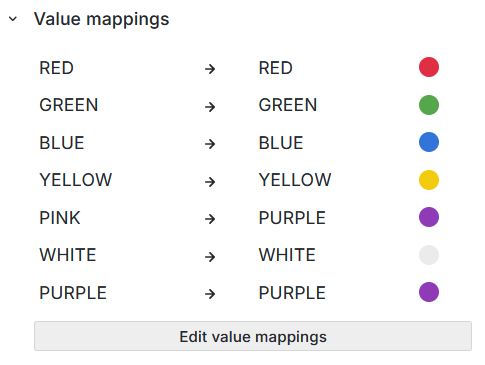
\includegraphics[scale=0.6]{imgs/grafana_value_mapping}
	\caption{Mapiranje vrijednosti LED dioda na boje}
	\label{fig:grafana_value_mapping}
\end{figure}

Podaci svih prikazanih panela dobiveni su iz kante \textit{esp32state}. Sljedeći je upit korišten za prikaz stanja tijekom vremena. Za vremenski raspon koristi varijable za početak i kraj odabranog vremenskog okvira u Grafani koje nudi \engl{plugin} za bazu InfluxDB. Vrijednost za identifikator uređaja dobiva se iz varijable nadzorne ploče. 

\begin{lstlisting}[caption={Upit za dohvat stanja LED diode u vremenskom okviru}, language=flux]
from(bucket: "esp32state")
|> range(start: v.timeRangeStart, stop: v.timeRangeStop)
|> filter(fn: (r) => r._measurement == "esp32")
|> filter(fn: (r) => r.device_id == "${device_id}")
|> map(fn: (r) => ({ color: r._value, time: r._time }))
\end{lstlisting}

Sljedeće slike prikazuju red sa senzorskim očitanjima. Prva tri panela sa slike \ref{fig:grafana_data_1} prikazuju trenutno izmjerene senzorske vrijednosti, dok drugi panel prikazuje temperaturu tijekom vremena. Isto tako, moguće je primijetiti kako su trenutna mjerenja drukčije obojana. Definirane su granične vrijednosti \engl{thresholds} na temelju kojih se evaluira koje će boje biti panel. Boja simbolizira kritičnost stanja u kojem se uređaj nalazi. Žuta boja signalizira upozorenje, dok crvena predstavlja ozbiljno stanje izmjerene vrijednosti. Ostala dva panela na slici \ref{fig:grafana_data_2} prikazuju vlažnost zraka i vlagu zemlje kroz vrijeme. Na dnu svakog linijskog grafa vidljiv je i serijski broj uređaja, stoga ukoliko je odabrano više uređaja, moguće je i dalje zaključiti koje su vrijednosti vezane za pojedini uređaj. Isto tako, na svakom je panelu odabrana prikladna mjerna jedinica. 

\begin{figure}[ht]
	\centering
	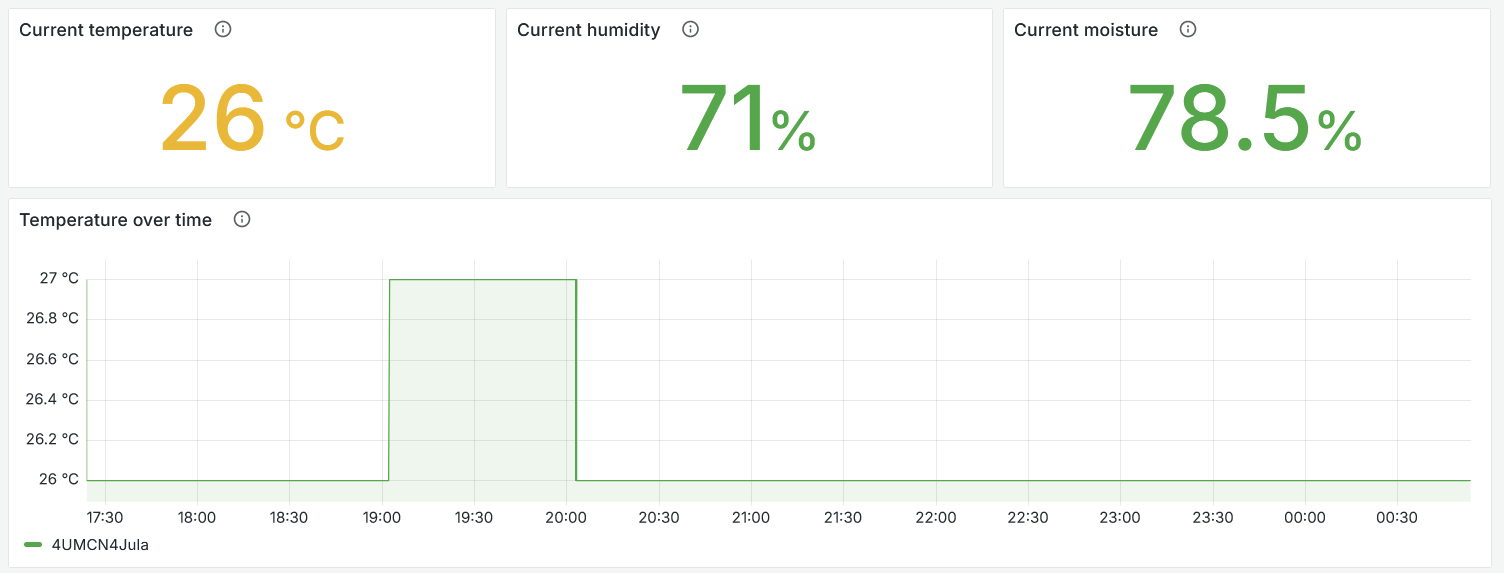
\includegraphics[scale=0.4]{imgs/grafana_data_1}
	\caption{Trenutno izmjerena senzorska mjerenja i temperatura kroz vrijeme}
	\label{fig:grafana_data_1}
\end{figure}

\begin{figure}[ht]
	\centering
	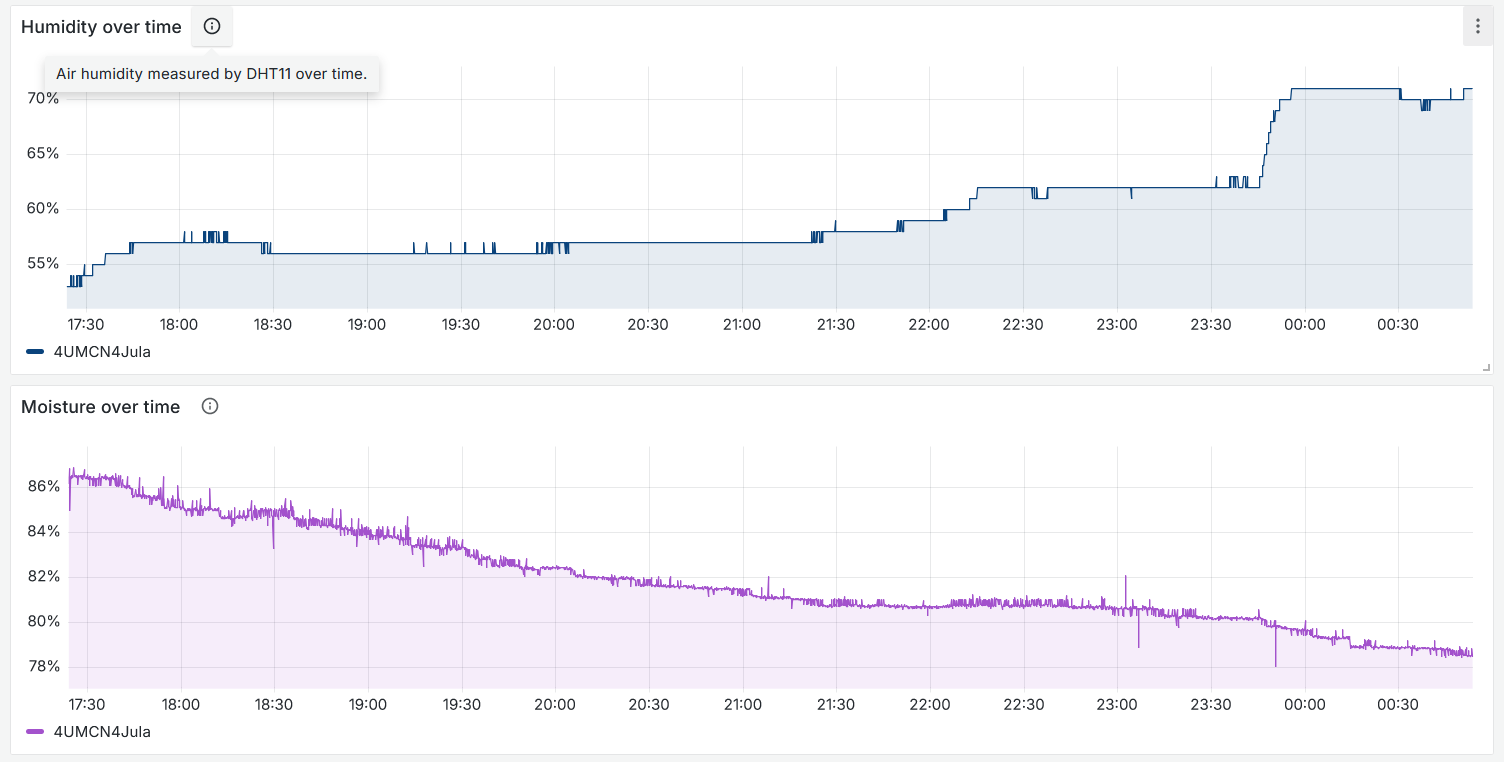
\includegraphics[scale=0.4]{imgs/grafana_data_2}
	\caption{Vlažnost zraka i zemlje kroz vrijeme}
	\label{fig:grafana_data_2}
\end{figure}

Sljedeći programski isječak prikazuje upit za dohvat temperature kroz vrijeme. Kao što je ranije spomenuto, koristi se kanta \textit{esp32data} za izvor podataka o senzorskim očitanjima. Grupiranje po serijskom broju uređaja važno je za točan prikaz podataka. Funkcijom \lstinline|keep()| zadržani su stupci za vrijeme, uređaj te sama vrijednost odabrane temperature, dok su ostali stupci automatski odbačeni.

\begin{lstlisting}[caption={Upit za dohvat temperature}, language=flux]
from(bucket: "esp32data")
|> range(start: v.timeRangeStart, stop: v.timeRangeStop)
|> filter(fn: (r) => r._measurement == "esp32" and r._field == "temperature")
|> filter(fn: (r) => r.device_id == "${device_id}")
|> group(columns: ["device_id"])
|> keep(columns: ["_time", "_value", "device_id"])
\end{lstlisting}

Slika \ref{fig:thresholds} prikazuje ranije spomenute granične vrijednosti za stiliziranje panela. Ove se vrijednosti odnose na panel s trenutnim senzorskim mjerenjem temperature. Srednja granica jest 25°C, dok je kao gornja granica postavljena 30°C. Sve vrijednosti ispod srednje granice označene su zelenom bojom te se smatraju prihvatljivima.

\begin{figure}[ht]
	\centering
	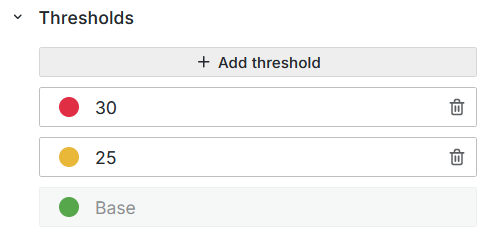
\includegraphics[scale=0.7]{imgs/thresholds}
	\caption{Granične vrijednosti za temperaturu zraka}
	\label{fig:thresholds}
\end{figure}

\subsection{Alarmni sustav}

Korisnici ne prate uvijek stanje uređaja niti očitanja mjerenih senzora, stoga je korisno slati obavijesti korisniku pri svakom neželjenom očitanom stanju. Grafana nudi alarmni sustav \engl{alerting system} koji omogućuje definiranje uvjeta pod kojima se generiraju obavijesti, na temelju podataka i metrika prikupljenih iz različitih izvora podataka. Mogu se kreirati pravila za alarme, postaviti pragovi za različita mjerenja, kao i definirati vremenski intervali za provjeru tih uvjeta. Kada su uvjeti ispunjeni, Grafana može poslati obavijesti putem raznih kanala, od kojih su neki e-pošta, Slack i Discord.  

Alarmni sustav omogućuje proaktivno praćenje performansi i dostupnosti sustava, osiguravajući pravovremenu obaviještenost o potencijalnim problemima. Isto tako, moguće je detaljno konfigurirati obavijesti, uključujući opcije za ponavljanje alarma i kreiranje eskalacijskih lanaca kako bi se osiguralo da obavijest dosegne tražene osobe. Povijest alarma se pohranjuje i može se pregledavati, što olakšava analizu i rješavanje problema \cite{grafana}. 

Dijagram na slici \ref{fig:alerting_system} prikazuje princip rada alarmnog sustava na Grafani. Alarmni sustav Grafane periodički ispituje izvore podataka i procjenjuje uvjet zapisan u pravilu alarma. Ako je uvjet prekršen, uključi se alarm za pojedinu instancu koja je prouzrokovala alarm. Šalju se obavijesti za aktivirane i razriješene alarme direktno kontakt točki ili prolaze notifikacijsku politiku za detaljnije preusmjeravanje. Alarmi se također mogu pridružiti panelima na nadzornim pločama za jednostavniji pregled alarma. 

Grafanin alarmni sustav sastoji se od dvije ključne komponente:
\begin{itemize}
	\item generator alarma: procjenjuje pravila i šalje aktivne ili razriješene alarme primatelju alarma, 
	\item primatelj alarma (\textit{Alertmanager}): prima alarme, odgovoran za njihovo rukovanje i slanje obavijesti.
\end{itemize}

\begin{figure}[ht]
	\centering
	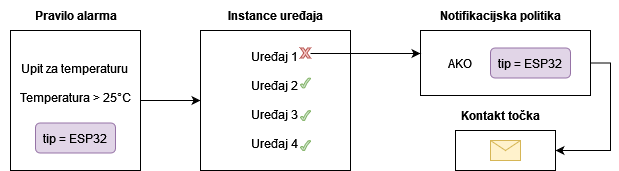
\includegraphics[scale=0.6]{imgs/alerting_system}
	\caption{Princip rada alarmnog sustava na Grafani \cite{grafana}}
	\label{fig:alerting_system}
\end{figure}

U nastavku su pobliže objašnjeni pojmovi ključni za razumijevanje alarmnog sustava.

Pravilo alarma \engl{alert rule} sastoji se od jednog ili više upita i izraza koji odabiru podatke koji se žele mjeriti. Također sadrži uvjet, a to je prag koji pravilo alarma mora ispuniti ili premašiti da bi se aktivirao. Unutar pravila alarma potrebno je odabrati točku kontakta ili notifikacijsku politiku kako bi se odredio način slanja obavijesti. Svako pravilo alarma može proizvesti više instanci, i svako pojavljivanje pravila naziva se alarm. Alarm se generira za svaku vremensku seriju, što je korisno jer se time omogućava praćenje više uređaja samo jednim pravilom. Ako su podaci grupirani po identifikatoru uređaja, alarm će se aktivirati za svaki pojedini identifikator. Pravila se često procjenjuju i njihova se stanja sukladno ažuriraju. Sustav obavještava isključivo o instancama koje ispunjavaju uvjete ili na koji su upravo razriješeni \engl{resolved}. 

Svako pravilo alarma mora imati evaluacijsku grupu te period čekanja \engl{pending period}. Svaka evaluacijska grupa ima razdoblje evaluacije odnosno procjene, i određuje koliko se često alarm procjenjuje. Period čekanja definira koliko dugo uvjet mora biti ispunjen prije nego se alarm pokrene, što smanjuje mogućnost lažno pozitivnih alarma. Period čekanja se isto tako može postaviti na nulu, čime se alarm efektivno pokreće odmah čim je uvjet ispunjen. Slika \ref{fig:alerting_resolved} prikazuje promjene stanja alarma i obavijesti koje se šalju u svakom stanju. Početno je normalno stanje kada uvjet nije ispunjen i alarm nije pokrenut. Kada se uvjet ispuni, alarm prelazi u stanje čekanja \engl{pending} dok period čekanja ne istekne. Na kraju perioda, ako je uvjet i dalje ispunjen, alarm prelazi u aktivno stanje i šalje obavijesti o promjeni stanja. Po završetku ispunjavanja uvjeta, alarm je razriješen i vraća se u normalno stanje, te se šalje obavijest o razrješenju alarma. Isto tako, ako je alarm u stanju čekanja, a uvjet se prestane ispunjavati tokom perioda čekanja, alarm se vraća u početno normalno stanje. 

\begin{figure}[ht]
	\centering
	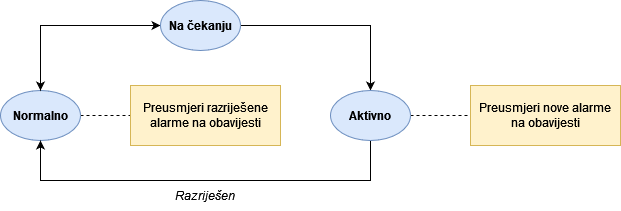
\includegraphics[scale=0.6]{imgs/alerting_resolved}
	\caption{Promjena stanja alarma \cite{grafana}}
	\label{fig:alerting_resolved}
\end{figure}

Notifikacijske politike pružaju fleksibilan način preusmjeravanja obavijesti. One usmjeravaju alarme na točke kontakta pomoću uparivanja oznaka \engl{label matching} s alarma. Notifikacijske politike nisu lista, nego stablasta struktura, čiji je korijen zadana notifikacijska politika te iz nje proizlaze mnoge politike. Svaka politika ima skup oznaka na temelju kojih se uparuje s kontaktnim točkama. Unutar alarma definiraju se oznake koje se nakon aktiviranja alarma uparuju s notifikacijskim politikama. Slika \ref{fig:label_matching} prikazuje princip uparivanja oznaka alarma s notifikacijskim politikama. Što je više oznaka definirano u alarmu, to dublje prolazi u strukturu notifikacijskih politika. Kako bi se odredilo koje notifikacijske politike trebaju rukovati alarmom, oznake se uparuju od početka stabla, odnosno zadane notifikacijske politike. Ona je uparena sa svim alarmima, što sprječava propuštanje preusmjeravanje alarma. Ako se pronađe podudarna politika, sustav nastavlja procjenjivati politike dublje u strukturi redom kojim su navedene. Ako je ugniježđena politika s alarmom, evaluiraju se i njezine podpolitike. Ovaj se proces odvija rekurzivno dok se ne dođe do najdublje politike u strukturi koja se podudara s oznakama alarma. U ovom slučaju, samo politika najdublje u strukturi obrađuje alarm. Ako alarm treba obraditi više politika, treba omogućiti uparivanje sa hijerarhijski srodnim odnosno sestrinskim pravilima na željenoj razini.  

\begin{figure}[ht]
	\centering
	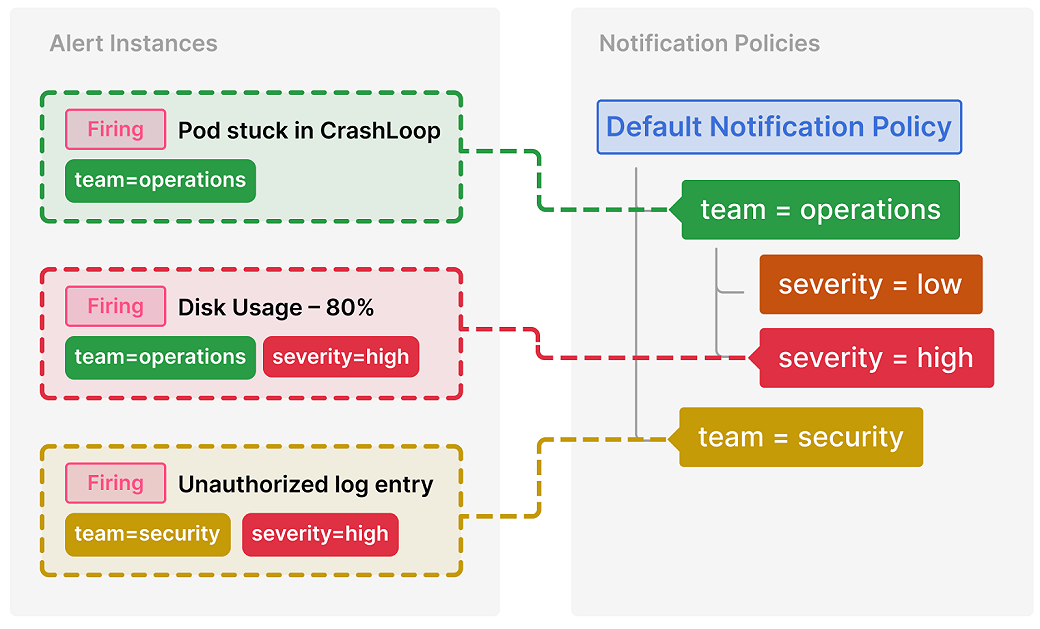
\includegraphics[scale=0.4]{imgs/label_matching}
	\caption{Uparivanje oznaka alarma i notifikacijskih politika \cite{grafana}}
	\label{fig:label_matching}
\end{figure}

Kao što je spomenuto, svaka je notifikacijska politika vezana za jednu točku kontakta \engl{contact point}. Točke kontakta sadrže konfiguraciju za slanje obavijesti o alarmima. To je popis integracija od kojih svaka šalje obavijest na određeni kanal. Grafana pruža integraciju s brojnim sustavima i aplikacijama za slanje pošte ili obavijesti. Unutar svake točke također se definira poruka obavijesti koja se šalje, a može koristiti unaprijed kreirane predloške ili poruku. Moguće je definirati i kontaktnu točku bez ikakve integracije, no u tom slučaju ona ne šalje nikakve obavijesti. Slika \ref{fig:labels_and_notifs} prikazuje vezu notifikacijskih politika i točaka kontakta.

\begin{figure}[ht]
	\centering
	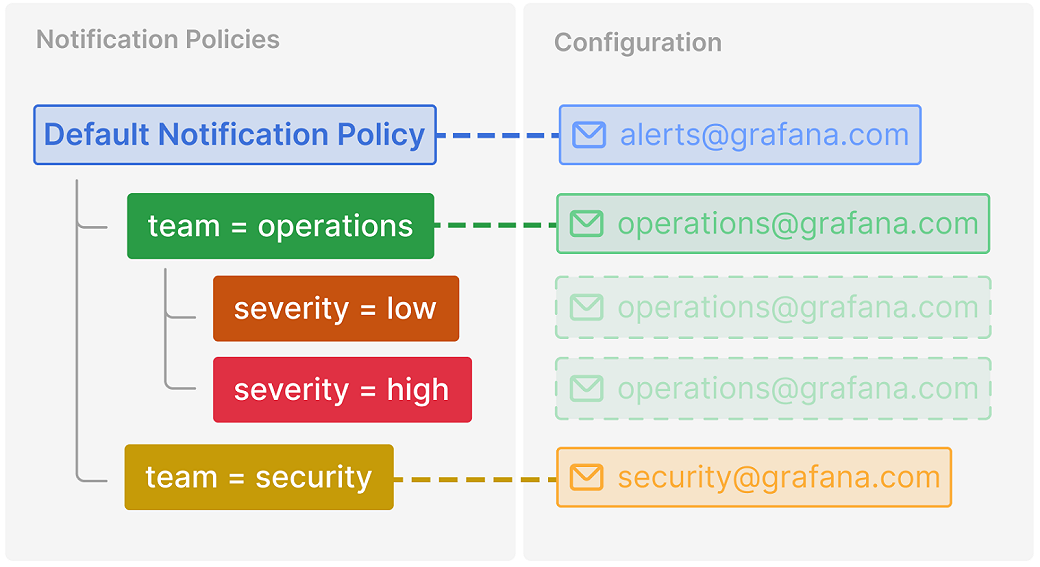
\includegraphics[scale=0.4]{imgs/labels_and_notifs}
	\caption{Uparivanje notifikacijskih oznaka i točaka kontakta \cite{grafana}}
	\label{fig:labels_and_notifs}
\end{figure}

Moguće je kreirati i predloške za slanje poruka u obavijesti. Za kreiranje predložaka koriste se predlošci programskog jezika Go. Naime, primatelj obavijesti odnosno komponenta \textit{Alertmanager} jest aplikacija napisana u programskom jeziku Go, te se kreirani predlošci prosljeđuju toj komponenti i izravno integriraju u njezin izvorni kod. Predlošci pružaju mogućnost definiranja strukture i sadržaja obavijesti o alarmima, čime postaju informativnije i prilagođenije potrebama. Važno je napomenuti kako postavljanjem predloška za točku kontakta sve obavijesti koje dolaze s te točke poprimaju oblik definiran predloškom. 

Predlošci se pišu koristeći sintaksu dvostrukih zagrada \lstinline|{{...}}| koje označavaju mjesta gdje će se dinamički umetnuti sadržaj. Unutar ovih zagrada mogu se koristiti različite naredbe poput varijabli, funkcija, petlji i uvjetnih izraza. Podaci se u predloške ubacuju kroz kontekst koji je struktura ili rječnik podataka proslijeđen predlošku pri njegovu izvršavanju. Unutar primatelja obavijesti, predložak se učitava i obrađuje, nakon čega se izvršava s određenim podacima pomoću posebnih funkcija izvršavanja. Pri izvršavanju, dinamički podaci zamjenjuju odgovarajuće oznake unutar predloška, generirajući konačni izlazni sadržaj. Sustav predložaka omogućuje i definiranje prilagođenih funkcija koje se mogu koristiti unutar predložaka. Ovo omogućuje proširenje funkcionalnosti predložaka dodavanjem specifičnih operacija koje se mogu izvršavati nad podacima, čime se povećava fleksibilnost cijelog sustava predložaka \cite{go_templating}. 

Sljedeći odsječak koda prikazuje primjer jednog predloška u programskom jeziku Go kakav bi se mogao naći u točki kontakta alarmnog sustava Grafane. Unutar definiranog predloška prolazi se po svim generiranim alarmima i za svaki alam iz popisa oznaka odabere se oznaka s ključem \textit{alertname}. Isto tako, provjerava se trenutno stanje alarma i na temelju dobivene varijable generira se ostatak poruke. 

\begin{lstlisting}[caption={Primjer predloška u programskom jeziku Go}, language=go]
{{ define "custom_alert_template" }}
	{{ range .Alerts }}
		This is my alert named {{ index .Labels "alertname" }}
		{{ if eq .Status "resolved" }}
			This alert is resolved.
		{{ else }}
			This alert is currently firing!
		{{ end }}
	{{ end }}
{{ end }}
\end{lstlisting}

Predlošci u jeziku Go prate određenu strukturu, te se varijable predloška mijenjaju podacima iz samog alarma. Sučelje za kreiranje predloška nudi i provjeru napisanog testirajući predložak nad testnim alarmom. Također je moguće verificirati valjanost predloška s podacima iz trenutno aktivnog alarma. Slika \ref{fig:grafana_templating} prikazuje testiranje gornjeg predloška nad kreiranim testnim alarmom. Alarmi su podaci u formatu JSON koji se dinamički učitaju u taj predložak.

\begin{figure}[ht]
	\centering
	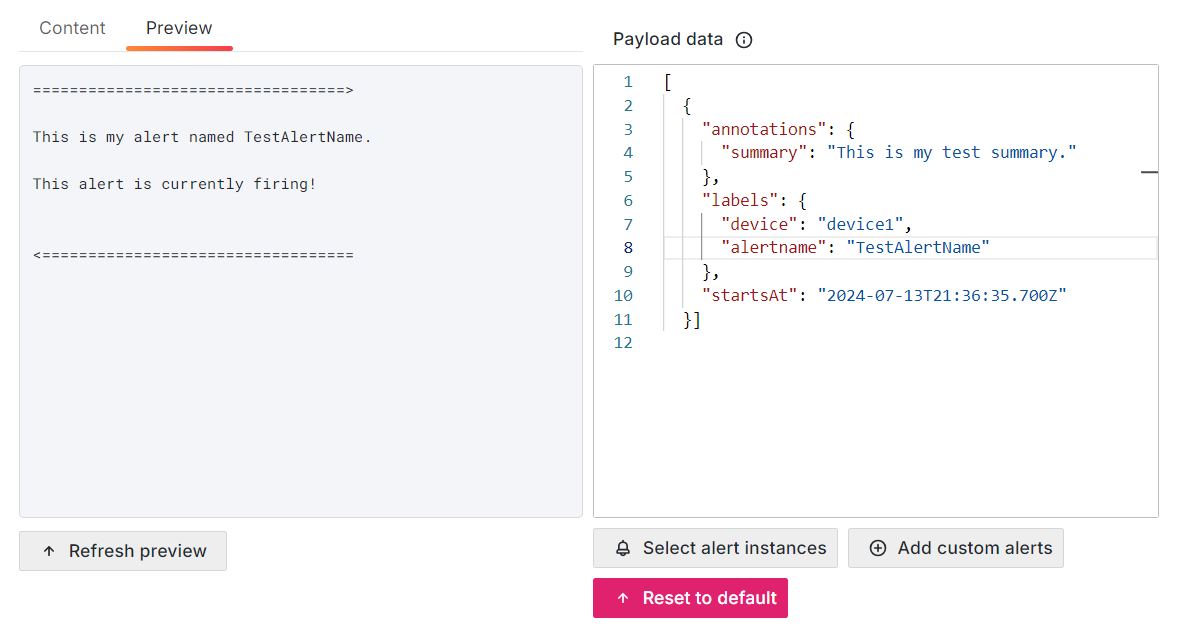
\includegraphics[scale=0.4]{imgs/grafana_templating}
	\caption{Primjer testiranja predloška nad probnim alarmom}
	\label{fig:grafana_templating}
\end{figure}

Za potrebe razvijenog sustava kreirano su dva alarma: alarm za vlažnost tla te alarm kada u bazi nema novih podataka duži vremenski period. Najprije je kreiran alarm kada je u kanti \textit{esp32state} vrlo malo ili nema uopće podataka u posljednjih deset minuta. Alarm je kreiran pomoću sljedećeg upita:

\begin{lstlisting}[caption={caption text}, language=flux]
from(bucket: "esp32state")
|> range(start: v.timeRangeStart, stop: v.timeRangeStop)
|> filter(fn: (r) => r._measurement == "esp32")
|> group(columns: ["device_id"])
|> count()
|> group(columns: ["device_id"])
|> map(fn: (r) => ({ 
	_value: r._value,
	device_id: r.device_id
}))
|> yield(name: "count")
\end{lstlisting}

Upit je vrlo sličan ranijem upitu za dohvat podatkovnih točaka, no razlika jest što sljedeći upit vraća isključivo broj pronađenih točaka. Ako se u kanti nalazi manje od pet točaka, ili ako ih nema uopće, alarm se aktivira. Također je postavljeno aktiviranje alarma ako upit ne vrati nikakvu vrijednost, ili vrati praznu vrijednost. Evaluacijski period je pet minuta, te uvjet mora biti ispunjen još sljedećih pet minuta kako bi se alarm aktivirao. Slika \ref{fig:alert_rule_esp32state} prikazuje kreirani alarm. Alarmu su dodijeljene dvije oznake: jedna za vrstu uređaja, dok druga definira primatelja alarma. Notifikacijska politika povezuje ovu oznaku sa kontaktnom točkom. Alarm je također moguće utišati na željeni vremenski period. Utišanja alarma \engl{alert silences} stvaraju se na temelju oznaka i imena alarma. Obavezno je definirati trajanje utišanja budući da nije moguće neograničeno utišati alarme. 

\begin{figure}[ht]
	\centering
	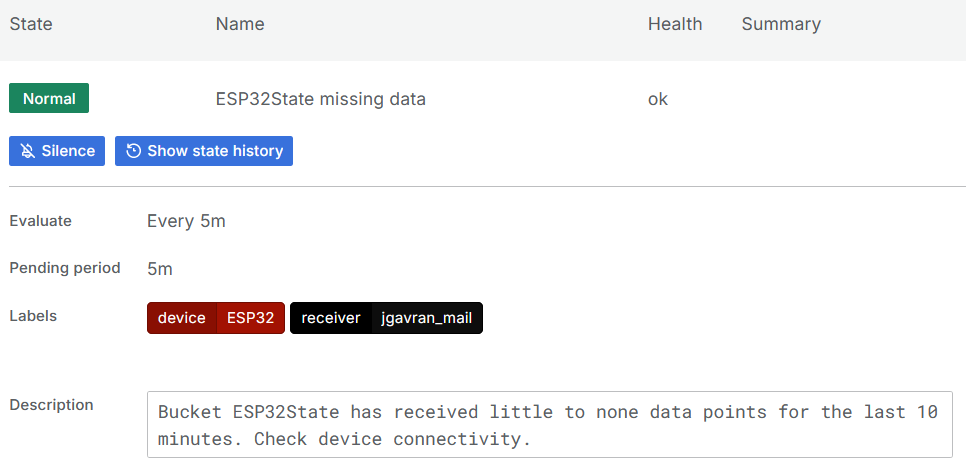
\includegraphics[scale=0.6]{imgs/alert_rule_esp32state}
	\caption{Alarm za podatke koji nedostaju posljednjih deset minuta}
	\label{fig:alert_rule_esp32state}
\end{figure}

Na slici \ref{fig:alert_rule_esp32state_states} nalaze se stanja alarma kroz vrijeme. Vremenski najstarije stanje prikazano je na dnu tablice stanja. Kao što je vidljivo na slici, alarm je bio aktivan određeni vremenski period. Oznaka \textit{Nodata} indikator je da je alarm aktiviran jer upit nije vratio nikakav rezultat, što je također znak da se u kanti ne nalaze nikakvi podaci. Nakon toga je alarm pauziran, čime se vratio u normalno stanje. Nakon toga je ponovno pokrenut, te budući da se u idućih pet minuta u bazi nisu pojavili nikakvi podaci, alarm prelazi u stanje čekanja označeno žutom bojom. Po isteku vremena čekanja alarm se ponovno aktivirao. 

\begin{figure}[ht]
	\centering
	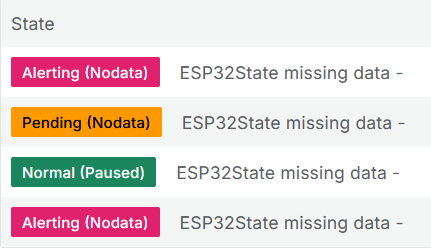
\includegraphics[scale=0.6]{imgs/alert_rule_esp32state_states}
	\caption{Promjena stanja alarma za podatke}
	\label{fig:alert_rule_esp32state_states}
\end{figure}

Slika \ref{fig:notif_policy} sadrži prikaz notifikacijskih politika. Vidljiva je ugniježđena stablasta struktura politika. Isto tako, na dnu se nalazi nova notifikacijska politika koja sve alarme s oznakom primatelja postavljenom na \textit{jgavran\_mail} preusmjerava na kontaktnu toočku \textit{jgavran\_mail}. Ta kontaktna točka sadrži popis adresa e-pošte na koje se šalje obavijest o alarmu. 

\begin{figure}[ht]
	\centering
	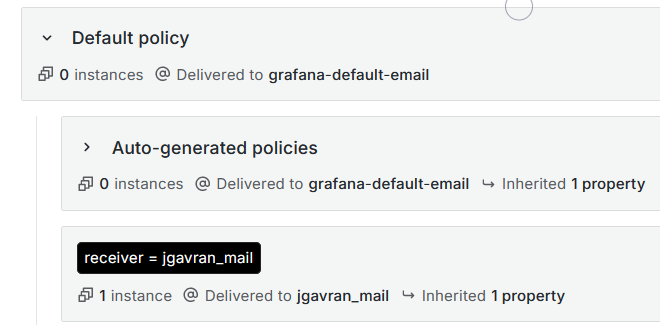
\includegraphics[scale=0.6]{imgs/notif_policy}
	\caption{Popis notifikacijskih politika i pripadajućih oznaka}
	\label{fig:notif_policy}
\end{figure}

Kreirani su predlošci za naslov i tijelo obavijesti alarma. Kao što je ranije opisano, korišteni su predlošci programskog jezika Go. Svaka poruka e-pošte koja se pošalje putem točke kontakta formatirana je na temelju kreiranog predloška. U nastavku su navedeni predlošci za naslov i tijelo poruke. Predložak za naslov je jednostavan, te osim naziva alarma sadrži jedino provjeru je li poslana obavijest o aktivaciji ili razrješenju alarma. S druge strane, predložak za tijelo koristi puno više sadržaja samog alarma za generiranje obavijesti. Na početku samog predloška definirane su varijable za poruku, sažetak i opis alarma. Sve tri varijable su navedene jer postoji mogućnost da će kreirani alarm imati jedno ili pak više od opisnih polja, stoga je važno uzeti u obzir sve opcije. Nakon toga, ovisno o tome postoje li varijable ili ne, uključuju se u predložak. Budući da je alarme moguće pridružiti nadzornim pločama, ako je navedenom alarmu pridružen panel odnosno nadzorna ploča, prikazat će se izravna poveznica na ploču. Nadalje se prikazuju sve oznake definirane u alarmu kao i vrijednosti samih izraza korištenih u alarmu kako bi obavijest bila potpunog sadržaja i kako bi korisnik zaključio je li potrebno brzo reagirati na obavijest.

\begin{lstlisting}[caption={Predlošci za naslov i tijelo obavijesti alarma}, language=go]
{{ define "jgavran_title_template" }}
	{{ range .Alerts }}
		{{if eq .Status "resolved" }}
		[OK] {{ index .Labels "alertname" }}
		{{ else }}
		[FIRING] {{ index .Labels "alertname" }}
		{{ end }}
	{{ end }}
{{ end }}

{{ define "jgavran_body_template" }}

{{ range .Alerts }}

	{{- $message := index .Annotations "message" -}}
	{{- $summary := index .Annotations "summary" -}}
	{{- $description := index .Annotations "description" -}}
	
	{{- if $message }}
	{{$message -}}
	{{ end }}
	{{- if $summary }}
	{{$summary -}}
	{{ end }}
	{{- if $description }}
	{{$description -}}
	{{ end }}
	
	Dashboard: {{ .DashboardURL }}
	Labels:
	{{ range .Labels.SortedPairs -}}
		- {{ .Name }} = {{ .Value }}
	{{ end }}
	Values:
		{{ .ValueString }}
	
{{ end }}

{{ end }}
\end{lstlisting}

Sljedeća slika prikazuje obavijest dobivenu na temelju opisanog alarma koji je preusmjeren na točku kontakta e-pošte i zatim obrađen gornjim predloškom. Iz naslova je moguće vidjeti kako je alarm razriješen, a u samom tijelu nalaze se detaljnije informacije o samom alarmu. 

\begin{figure}[ht]
	\centering
	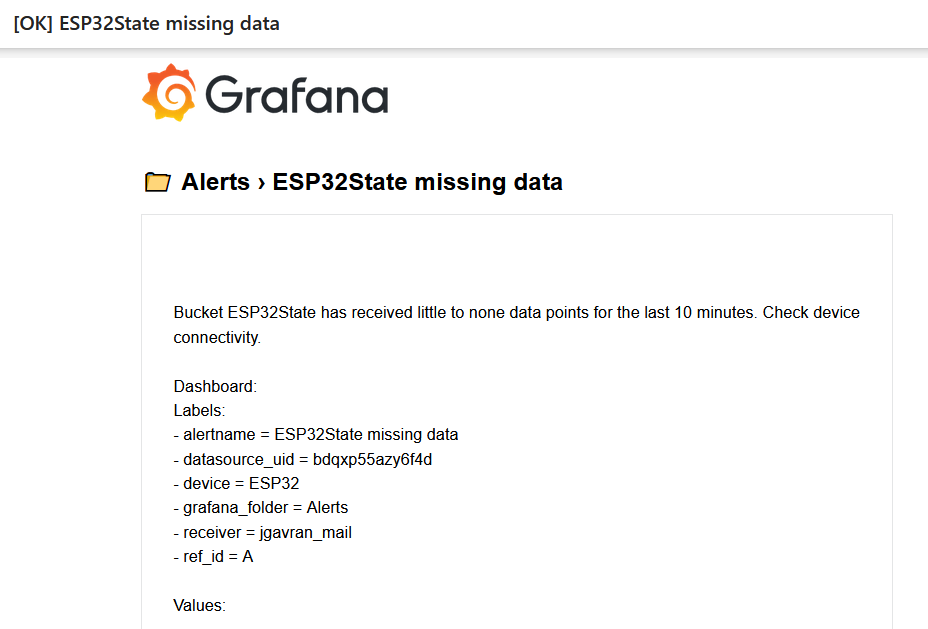
\includegraphics[scale=0.6]{imgs/alert_mail}
	\caption{E-pošta o razriješenom alarmu}
	\label{fig:alert_mail}
\end{figure}

Kao što je već spomenuto, alarmi se mogu pridružiti pojedinim panelima. Tako je kreiran alarm za senzorsko očitanje vlažnosti tla i pridružen je pripadnom linijskom vremenskom grafu. Važno je napomenuti kako se alarmi mogu pridružiti samo panelima koji prikazuju vremenske serije. Upit za vlažnost tla dohvaća samo posljednje vrijednosti za svaki uređaj i u postavkama alarma izraz se evaluira svakih deset sekundi, što je ujedno i minimalno dozvoljeni evaluacijski period. Period čekanja odnosno vremenski okvir u kojem uvjet mora biti ispunjen jest jedna minuta. Periodi su postavljeni tako nisko radi jednostavnijeg testiranja alarma, no nakon provjere valjanosti alarma jednostavno ih je prilagoditi. Kao granica prihvatljivosti vlažnosti zemlje uzeta je vrijednost od 20\%. Na slici \ref{fig:moisture_alert} nalazi se ranije prikazan graf za vlažnost tla kroz vrijeme, no ovaj mu je put pridružen alarm. Ikona srca pokraj naziva panela upućuje da je alarm vezan za njega. Na grafu je vidljivo kako je na početku vlažnost tla jednaka nuli, stoga je poslije prve evaluacije nakon kreiranja alarma alarm promijenio stanje u čekanje, što je označeno okomitom žutom crtom. Nakon isteka perioda čekanja, a vlažnost tla je i dalje ispod dozvoljene vrijednosti, alarm prelazi u aktivno stanje. Aktivacija alarma signalizira se crvenom okomitom crtom. Vlažnost tla je zatim promijenila vrijednost u otprilike 50\%, zbog čega je stanje alarma nakon jedne minute vraćeno u normalno, i to se očituje okomitom zelenom crtom.

\begin{figure}[ht]
	\centering
	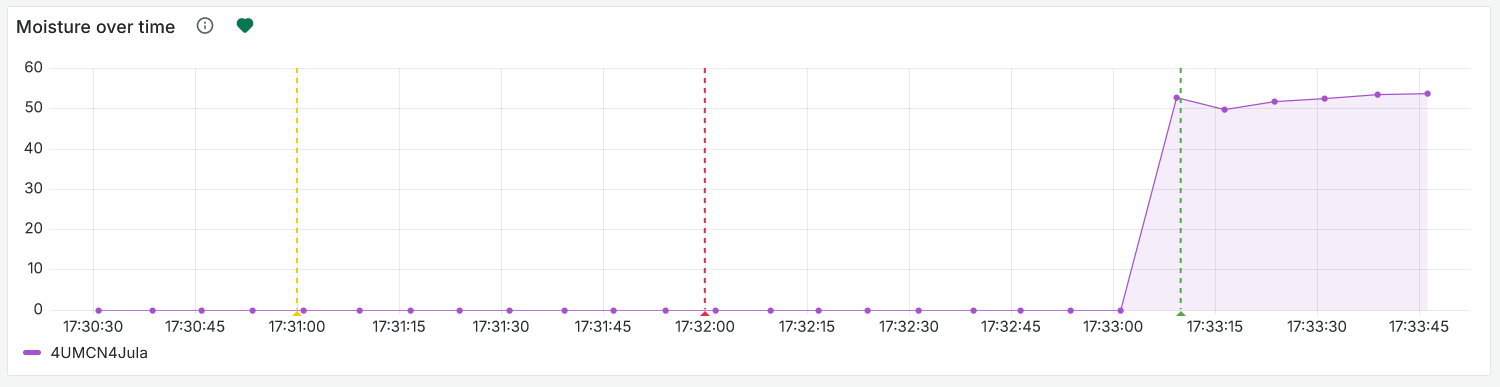
\includegraphics[scale=0.4]{imgs/moisture_alert}
	\caption{Alarm za vlažnost tla kroz vrijeme}
	\label{fig:moisture_alert}
\end{figure}

Sljedeće dvije slike \ref{fig:firing_low_moisture} i \ref{fig:ok_low_moisture} prikazuju obavijesti dobivene pri aktivaciji i razrješenju alarma. Vrijednosti izraza A i B odnose se na strukturu samog alarma. Izraz A jest vrijednost samog upita, dok je izraz B procjena postavljenog uvjeta. Iz prve se obavijesti može vidjeti da je vrijednost izraza A bila jednaka nuli, što je vidljivo i na gornjem grafu. Budući da je uvjet postavljen u izrazu B zadovoljen, odnosno vrijednost izraza A je manja od 20, vrijednost izraza B jednaka je jedinici, što signalizira aktivaciju alarma. S druge strane, u obavijesti razrješenja alarma vrijednost izraza A jednaka je 52.68, što je više od postavljenog uvjeta izraza B, stoga je njegova vrijednost jednaka nuli. 

\begin{figure}[ht]
	\begin{minipage}[t]{0.4\textwidth}
		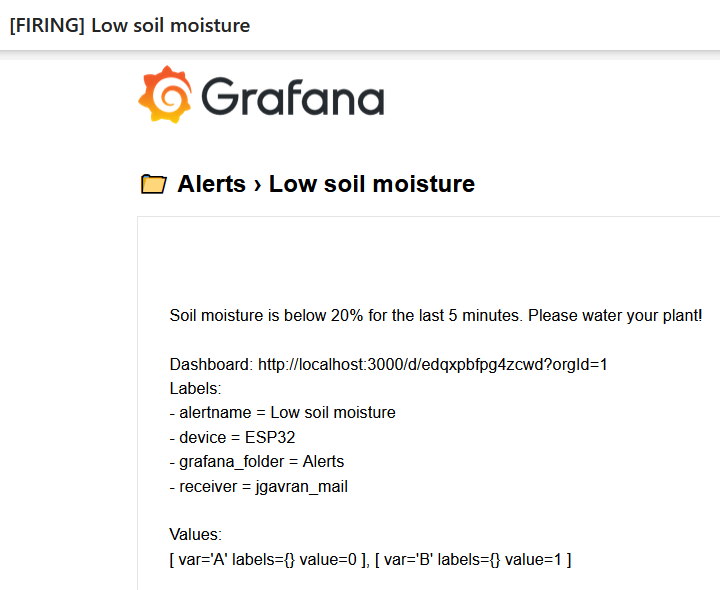
\includegraphics[width=\linewidth]{imgs/firing_low_moisture}
		\caption{Obavijest o aktivaciji alarma niske vlažnosti tla}
		\label{fig:firing_low_moisture}
	\end{minipage}
	\hspace*{\fill}
	\begin{minipage}[t]{0.4\textwidth}
		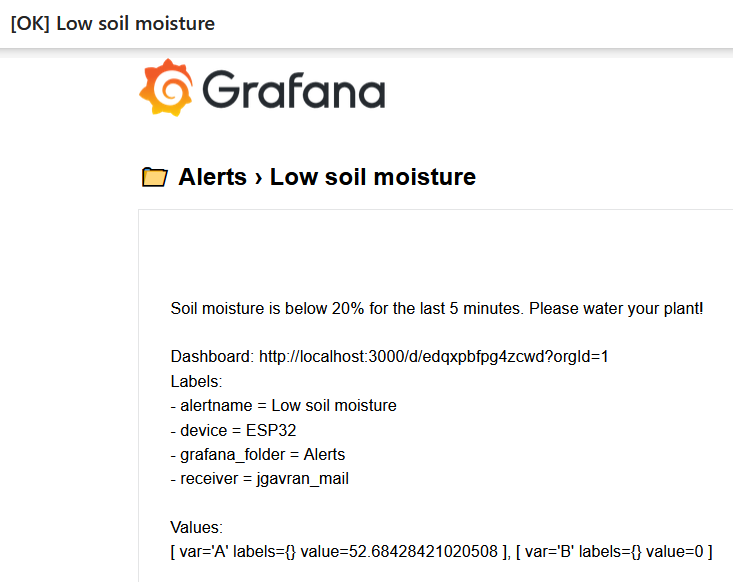
\includegraphics[width=\linewidth]{imgs/ok_low_moisture}
		\caption{Obavijest o razrješenju alarma niske vlažnosti tla}
		\label{fig:ok_low_moisture}
	\end{minipage}
\end{figure}

Alarmi se mogu sukladno napraviti za vlagu i temperaturu zraka. Preporuča se kreirati odvojene alarme za sva senzorska očitanja kako bi imali različite granične vrijednosti. Isto tako, ako korišteni uređaji prate drukčije uvjete gdje su granične vrijednosti različite od postavljenih, moguće je kreirati i alarme specifične uređajima. Potrebno je samo u upit alarma navesti specifičan uređaj nad kojim se ispituju podaci. 

Osim e-pošte, alarmi se mogu preusmjeravati na različite kanale i mobilne aplikacije koje podržavaju obavještavanje. Aplikacije koje se često koriste za slanje obavijesti su PagerDuty i Opsgenie. To su vodeće aplikacije za upravljanje incidentima i obavještavanje koje pomažu organizacijama da odgovore na kritične probleme i smanje vrijeme odgovora na incident. Aplikacije se jednostavno integriraju s različitim sustavima za praćenje i omogućavaju definiranje složenih pravila obavještavanja i automatizaciju eskalacijskih postupak. Osim \textit{push} notifikacijama, aplikacije mogu slati obavijesti i putem SMS poruke te poziva, ovisno o definiranoj eskalacijskoj politici \cite{pagerduty_vs_opsgenie}. Navedene aplikacije mogu se integrirati s Grafanom pomoću API ključa kreiranog u aplikaciji. Tako se obavijesti o promjenama stanja u razvijenom sustavu mogu detaljnije i pozornije pratiti. 

\eject
\chapter{Zaključak}

Moj zaključak.

\eject

\bibliography{literatura}{}
\bibliographystyle{fer}

\title{Sustav za udaljeni nadzor u poljoprivredi temeljen na platformi ESP32-C3 i AWS-uslugama}
\begin{sazetak}
Ovo je moj hrvatski sažetak.

\kljucnerijeci{IoT, ESP32-C3-DevKitM-1, AWS, MQTT, InfluxDB, Grafana, računarstvo u oblaku, precizna poljoprivreda}
\end{sazetak}

% TODO: Navedite naslov na engleskom jeziku.
\engtitle{System For Remote Monitoring In Agriculture Based On ESP32-C3 Platform and AWS Services}
\begin{abstract}
This is my english abstract.

\keywords{IoT, ESP32-C3-DevKitM-1, AWS, MQTT, InfluxDB, Grafana, cloud computing, precision agriculture}
\end{abstract}

\end{document}
